\documentclass[11pt,a4paper]{article}
\usepackage[margin=16mm]{geometry}
\usepackage{tikz,amsmath,booktabs,lmodern,graphicx}
\usetikzlibrary{arrows.meta}
\setlength{\parindent}{0pt}
\begin{document}
{\LARGE\bfseries Family 1: grouped graph atlas}\par\vspace{3mm}
{\large Exact reachable sizes $1$ through $20$}\par\vspace{4mm}
Each vertex has two outgoing edges and unrestricted indegree. Loops and parallel edges are allowed. Arrows have identical styles: their local port order is immaterial. Vertex numbers identify possible starting states.\par\vspace{2mm}
For a chosen start, $H(G)$ is the shortest positive length of two distinct equal-length words whose endpoint vectors agree for every static mask. Different starting states are scored separately. A double circle marks an alternative start, never a simultaneous collection of roots.\par\vspace{3mm}
\begin{center}\small\begin{tabular}{rcrrl}\toprule $m$ & $F(m)$ & Rooted winners & Shapes & Evidence \\\midrule
1 & $1$ & 1 & 1 & Certified complete \\
2 & $3$ & 1 & 1 & Certified complete \\
3 & $6$ & 2 & 1 & Certified complete \\
4 & $10$ & 1 & 1 & Certified complete \\
5 & $15$ & 5 & 4 & Certified complete \\
6 & $23$ & 2 & 1 & Certified complete \\
7 & $34$ & 8 & 4 & Certified complete \\
8 & $\ge35$ & -- & -- & Global maximum unresolved \\
9 & $\ge34$ & -- & -- & Constructive lower example \\
10 & $\ge34$ & -- & -- & Constructive lower example \\
11 & $\ge34$ & -- & -- & Constructive lower example \\
12 & $\ge34$ & -- & -- & Constructive lower example \\
13 & $\ge34$ & -- & -- & Constructive lower example \\
14 & $\ge34$ & -- & -- & Constructive lower example \\
15 & $\ge34$ & -- & -- & Constructive lower example \\
16 & $\ge34$ & -- & -- & Constructive lower example \\
17 & $\ge34$ & -- & -- & Constructive lower example \\
18 & $\ge34$ & -- & -- & Constructive lower example \\
19 & $\ge34$ & -- & -- & Constructive lower example \\
20 & $\ge34$ & -- & -- & Constructive lower example \\
\bottomrule\end{tabular}\end{center}\vspace{2mm}
For $m\le7$, the 20 certified maximizing rooted classes are grouped into 13 ordinary graph shapes. Every vertex giving one of those rooted classes is marked, including automorphically equivalent vertices. The source witnesses and full root-to-class mappings are preserved in the accompanying JSON.\par\vspace{2mm}
At $m=8$, the picture is the current heuristic leader: finder length $50$, estimated $H\approx49$ (rough range $48$--$50$), rigorous graph bound $1\le H\le50$. The independently certified global lower bound $F(8)\ge35$ comes from a different graph. No exact score or global maximality is claimed for the pictured graph.\par\vspace{2mm}
For $9\le m\le20$, a marked vertex is only the start of an example with $H\ge34$, proved by projection to a certified seven-state graph. These are not asserted to be winners.\par\vspace{2mm}
Exactly $m$ reachable vertices is distinct from a cumulative budget $1,\ldots,m$. Deleting unreachable vertices preserves all rooted trajectories and $H(G)$; the cumulative optimum is therefore the maximum over the exact reachable sizes. No strong connectivity assumption is imposed.
\clearpage
{\LARGE\bfseries $m=1$}\par\vspace{3mm}
Global maximum $F(1)=1$; all 1 rooted maximizing classes, grouped into 1 ordinary shape.\par\vspace{2mm}
Double-circled vertices are all optimal starting states. Choose one marked start at a time; each choice defines a separate rooted graph.\par\vspace{3mm}
\begin{minipage}[t]{.94\textwidth}\centering
\resizebox{10.3cm}{!}{% Family 1 rooted seed, m=1; key=0000.
% Requires \usepackage{tikz} and \usetikzlibrary{arrows.meta}.
% Score and global-maximality metadata belong in the surrounding caption.
\begin{tikzpicture}[x=1cm,y=1cm,
  f1atlas state/.style={circle,draw=black,fill=white,line width=.5pt,inner sep=0pt,font=\fontsize{7}{8}\selectfont},
  f1atlas root/.style={f1atlas state,double,double distance=.42mm},
  f1atlas port0/.style={-{Stealth[length=1.45mm,width=1.05mm]},draw=black,line width=.48pt},
  f1atlas port1/.style={f1atlas port0},
  f1atlas label/.style={font=\fontsize{6}{7}\selectfont,fill=white,inner sep=.4pt}
]
\path[use as bounding box] (-3,-3) rectangle (3,3);
% edge 0 0 0
\draw[f1atlas port0] (-0.20270,-0.00880) .. controls (-0.76121,-0.11454) and (0.15129,0.65405) .. (-0.05791,0.16668);
% edge 0 1 0
\draw[f1atlas port1] (0.04784,0.12164) .. controls (-0.15129,0.65405) and (0.76121,-0.11454) .. (0.24538,0.00878);
% state 0
\node[f1atlas root,minimum size=4.1538mm,fill=black!10] (q0) at (0.00000,-0.09231) {$ 0 $};
\end{tikzpicture}
}\par
\small\textbf{(a)} $H=1$. Optimal starts: $\{0\}$.\\1 distinct rooted maximizing class.\par\end{minipage}
\clearpage
{\LARGE\bfseries $m=2$}\par\vspace{3mm}
Global maximum $F(2)=3$; all 1 rooted maximizing classes, grouped into 1 ordinary shape.\par\vspace{2mm}
Double-circled vertices are all optimal starting states. Choose one marked start at a time; each choice defines a separate rooted graph.\par\vspace{3mm}
\begin{minipage}[t]{.94\textwidth}\centering
\resizebox{10.3cm}{!}{% Family 1 rooted seed, m=2; key=00010001.
% Requires \usepackage{tikz} and \usetikzlibrary{arrows.meta}.
% Score and global-maximality metadata belong in the surrounding caption.
\begin{tikzpicture}[x=1cm,y=1cm,
  f1atlas state/.style={circle,draw=black,fill=white,line width=.5pt,inner sep=0pt,font=\fontsize{7}{8}\selectfont},
  f1atlas root/.style={f1atlas state,double,double distance=.42mm},
  f1atlas port0/.style={-{Stealth[length=1.45mm,width=1.05mm]},draw=black,line width=.48pt},
  f1atlas port1/.style={f1atlas port0},
  f1atlas label/.style={font=\fontsize{6}{7}\selectfont,fill=white,inner sep=.4pt}
]
\path[use as bounding box] (-3,-3) rectangle (3,3);
% edge 0 0 0
\draw[f1atlas port0] (-0.20270,1.64697) .. controls (-0.76121,1.54122) and (0.15129,2.30982) .. (-0.05791,1.82245);
% edge 0 1 1
\draw[f1atlas port1] (-0.02946,1.34622) .. controls (-0.16367,0.35643) and (-0.16418,-0.62954) .. (-0.03101,-1.61171);
% edge 1 0 0
\draw[f1atlas port0] (0.02481,-1.65744) .. controls (0.16211,-0.64479) and (0.16573,0.34119) .. (0.03566,1.30048);
% edge 1 1 1
\draw[f1atlas port1] (-0.04029,-2.02055) .. controls (0.14442,-2.55282) and (-0.72661,-1.81916) .. (-0.21337,-1.92829);
% state 0
\node[f1atlas root,minimum size=4.1538mm,fill=black!10] (q0) at (0.00000,1.56346) {$ 0 $};
% state 1
\node[f1atlas root,minimum size=3.4615mm,fill=black!10] (q1) at (0.00000,-1.84038) {$ 1 $};
\end{tikzpicture}
}\par
\small\textbf{(a)} $H=3$. Optimal starts: $\{0, 1\}$.\\1 distinct rooted maximizing class.\par\end{minipage}
\clearpage
{\LARGE\bfseries $m=3$}\par\vspace{3mm}
Global maximum $F(3)=6$; all 2 rooted maximizing classes, grouped into 1 ordinary shape.\par\vspace{2mm}
Double-circled vertices are all optimal starting states. Choose one marked start at a time; each choice defines a separate rooted graph.\par\vspace{3mm}
\begin{minipage}[t]{.94\textwidth}\centering
\resizebox{10.3cm}{!}{% Family 1 rooted seed, m=3; key=000101020001.
% Requires \usepackage{tikz} and \usetikzlibrary{arrows.meta}.
% Score and global-maximality metadata belong in the surrounding caption.
\begin{tikzpicture}[x=1cm,y=1cm,
  f1atlas state/.style={circle,draw=black,fill=white,line width=.5pt,inner sep=0pt,font=\fontsize{7}{8}\selectfont},
  f1atlas root/.style={f1atlas state,double,double distance=.42mm},
  f1atlas port0/.style={-{Stealth[length=1.45mm,width=1.05mm]},draw=black,line width=.48pt},
  f1atlas port1/.style={f1atlas port0},
  f1atlas label/.style={font=\fontsize{6}{7}\selectfont,fill=white,inner sep=.4pt}
]
\path[use as bounding box] (-3,-3) rectangle (3,3);
% edge 0 0 0
\draw[f1atlas port0] (-0.20270,1.64697) .. controls (-0.76121,1.54122) and (0.15129,2.30982) .. (-0.05791,1.82245);
% edge 0 1 1
\draw[f1atlas port1] (0.11841,1.37896) .. controls (0.74790,0.39812) and (1.32828,-0.60665) .. (1.85953,-1.63534);
% edge 1 0 1
\draw[f1atlas port0] (2.13343,-1.76385) .. controls (2.44657,-1.29549) and (2.38675,-2.43275) .. (2.16423,-1.95755);
% edge 1 1 2
\draw[f1atlas port1] (1.78207,-1.81885) .. controls (0.59403,-1.67929) and (-0.57873,-1.67744) .. (-1.73623,-1.81328);
% edge 2 0 0
\draw[f1atlas port0] (-1.86570,-1.68481) .. controls (-1.22375,-0.68462) and (-0.64244,0.31954) .. (-0.12178,1.32767);
% edge 2 1 1
\draw[f1atlas port1] (-1.78207,-1.86172) .. controls (-0.59403,-2.00127) and (0.57873,-2.00313) .. (1.73623,-1.86728);
% state 0
\node[f1atlas root,minimum size=4.1538mm,fill=black!10] (q0) at (0.00000,1.56346) {$ 0 $};
% state 1
\node[f1atlas state,minimum size=3.4615mm] (q1) at (1.96542,-1.84038) {$ 1 $};
% state 2
\node[f1atlas root,minimum size=3.4615mm,fill=black!10] (q2) at (-1.96542,-1.84018) {$ 2 $};
\end{tikzpicture}
}\par
\small\textbf{(a)} $H=6$. Optimal starts: $\{0, 2\}$.\\2 distinct rooted maximizing classes.\par\end{minipage}
\clearpage
{\LARGE\bfseries $m=4$}\par\vspace{3mm}
Global maximum $F(4)=10$; all 1 rooted maximizing classes, grouped into 1 ordinary shape.\par\vspace{2mm}
Double-circled vertices are all optimal starting states. Choose one marked start at a time; each choice defines a separate rooted graph.\par\vspace{3mm}
\begin{minipage}[t]{.94\textwidth}\centering
\resizebox{10.3cm}{!}{% Family 1 rooted seed, m=4; key=0102000201030003.
% Requires \usepackage{tikz} and \usetikzlibrary{arrows.meta}.
% Score and global-maximality metadata belong in the surrounding caption.
\begin{tikzpicture}[x=1cm,y=1cm,
  f1atlas state/.style={circle,draw=black,fill=white,line width=.5pt,inner sep=0pt,font=\fontsize{7}{8}\selectfont},
  f1atlas root/.style={f1atlas state,double,double distance=.42mm},
  f1atlas port0/.style={-{Stealth[length=1.45mm,width=1.05mm]},draw=black,line width=.48pt},
  f1atlas port1/.style={f1atlas port0},
  f1atlas label/.style={font=\fontsize{6}{7}\selectfont,fill=white,inner sep=.4pt}
]
\path[use as bounding box] (-3,-3) rectangle (3,3);
% edge 0 0 1
\draw[f1atlas port0] (0.17993,0.76067) .. controls (0.72639,0.36593) and (1.32261,0.08669) .. (1.96861,-0.07705);
% edge 0 1 2
\draw[f1atlas port1] (0.02231,0.67074) .. controls (0.07193,0.13140) and (0.07343,-0.40420) .. (0.02681,-0.93608);
% edge 1 0 0
\draw[f1atlas port0] (2.04265,-0.02564) .. controls (1.47749,0.38262) and (0.88310,0.66578) .. (0.25947,0.82384);
% edge 1 1 2
\draw[f1atlas port1] (2.01355,-0.17987) .. controls (1.33847,-0.35408) and (0.73167,-0.63747) .. (0.19314,-1.03003);
% edge 2 0 1
\draw[f1atlas port0] (0.18542,-1.11984) .. controls (0.86049,-0.94563) and (1.46730,-0.66224) .. (2.00583,-0.26968);
% edge 2 1 3
\draw[f1atlas port1] (-0.16616,-1.10104) .. controls (-0.80989,-0.85920) and (-1.41819,-0.57757) .. (-1.99105,-0.25613);
% edge 3 0 0
\draw[f1atlas port0] (-2.01977,-0.07754) .. controls (-1.37709,0.16708) and (-0.78006,0.44565) .. (-0.22866,0.75818);
% edge 3 1 3
\draw[f1atlas port1] (-2.37472,-0.11475) .. controls (-2.89381,-0.33376) and (-2.21849,0.58324) .. (-2.29394,0.06398);
% state 0
\node[f1atlas root,minimum size=4.1538mm,fill=black!10] (q0) at (0.00222,0.88904) {$ 0 $};
% state 1
\node[f1atlas state,minimum size=3.4615mm] (q1) at (2.19231,-0.13374) {$ 1 $};
% state 2
\node[f1atlas state,minimum size=3.4615mm] (q2) at (0.00666,-1.16597) {$ 2 $};
% state 3
\node[f1atlas state,minimum size=3.4615mm] (q3) at (-2.19231,-0.14321) {$ 3 $};
\end{tikzpicture}
}\par
\small\textbf{(a)} $H=10$. Optimal starts: $\{0\}$.\\1 distinct rooted maximizing class.\par\end{minipage}
\clearpage
{\LARGE\bfseries $m=5$}\par\vspace{3mm}
Global maximum $F(5)=15$; all 5 rooted maximizing classes, grouped into 4 ordinary shapes.\par\vspace{2mm}
Double-circled vertices are all optimal starting states. Choose one marked start at a time; each choice defines a separate rooted graph.\par\vspace{3mm}
\begin{minipage}[t]{.48\textwidth}\centering
\resizebox{6.9cm}{!}{% Five-state extremal seed graph (a).
% Requires \usepackage{tikz} and \usetikzlibrary{arrows.meta}.
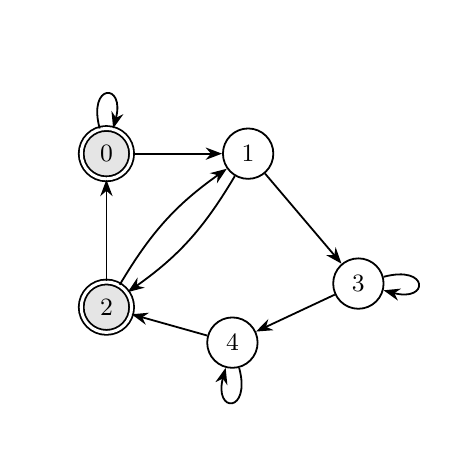
\begin{tikzpicture}[
  x=1cm,y=1cm,>=Stealth,
  f1m5 vertex/.style={circle,draw=black,line width=.65pt,minimum size=6.4mm,inner sep=0pt,font=\small},
  f1m5 root/.style={f1m5 vertex,double,double distance=1.1pt},
  f1m5 port zero/.style={->,draw=black,line width=.65pt},
  f1m5 port one/.style={->,draw=black,line width=.65pt},
  f1m5 label/.style={font=\scriptsize,fill=white,inner sep=1.1pt}
]
\path[use as bounding box] (-2.60,-2.65) rectangle (2.60,2.65);
\node[f1m5 root,fill=black!10] (q0) at (-1.60,1.05) {$ 0 $};
\node[f1m5 vertex] (q1) at (0.20,1.05) {$ 1 $};
\node[f1m5 root,fill=black!10] (q2) at (-1.60,-0.90) {$ 2 $};
\node[f1m5 vertex] (q3) at (1.60,-0.60) {$ 3 $};
\node[f1m5 vertex] (q4) at (0.00,-1.35) {$ 4 $};
% edge 0 0 0
\draw[f1m5 port zero] (q0) edge[loop above,min distance=6mm] (q0);
% edge 0 1 1
\draw[f1m5 port one] (q0) edge[] (q1);
% edge 1 0 2
\draw[f1m5 port zero] (q1) edge[bend left=12] (q2);
% edge 1 1 3
\draw[f1m5 port one] (q1) edge[] (q3);
% edge 2 0 0
\draw[f1m5 port zero] (q2) edge[] (q0);
% edge 2 1 1
\draw[f1m5 port one] (q2) edge[bend left=12] (q1);
% edge 3 0 3
\draw[f1m5 port zero] (q3) edge[loop right,min distance=6mm] (q3);
% edge 3 1 4
\draw[f1m5 port one] (q3) edge[] (q4);
% edge 4 0 2
\draw[f1m5 port zero] (q4) edge[] (q2);
% edge 4 1 4
\draw[f1m5 port one] (q4) edge[loop below,min distance=6mm] (q4);
\end{tikzpicture}
}\par
\small\textbf{(a)} $H=15$. Optimal starts: $\{0, 2\}$.\\2 distinct rooted maximizing classes.\par\end{minipage}
\hfill
\begin{minipage}[t]{.48\textwidth}\centering
\resizebox{6.9cm}{!}{% Five-state extremal seed graph (e).
% Requires \usepackage{tikz} and \usetikzlibrary{arrows.meta}.
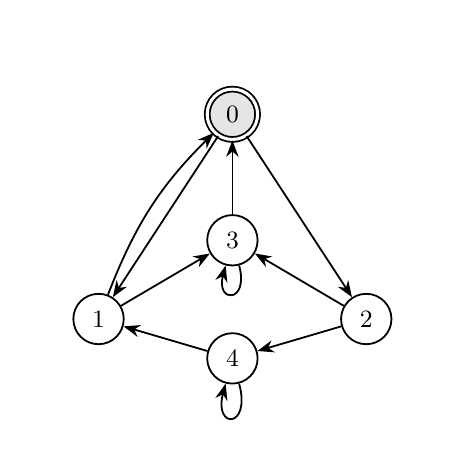
\begin{tikzpicture}[
  x=1cm,y=1cm,>=Stealth,
  f1m5 vertex/.style={circle,draw=black,line width=.65pt,minimum size=6.4mm,inner sep=0pt,font=\small},
  f1m5 root/.style={f1m5 vertex,double,double distance=1.1pt},
  f1m5 port zero/.style={->,draw=black,line width=.65pt},
  f1m5 port one/.style={->,draw=black,line width=.65pt},
  f1m5 label/.style={font=\scriptsize,fill=white,inner sep=1.1pt}
]
\path[use as bounding box] (-2.60,-2.65) rectangle (2.60,2.65);
\node[f1m5 root,fill=black!10] (q0) at (0.00,1.55) {$ 0 $};
\node[f1m5 vertex] (q1) at (-1.70,-1.05) {$ 1 $};
\node[f1m5 vertex] (q2) at (1.70,-1.05) {$ 2 $};
\node[f1m5 vertex] (q3) at (0.00,-0.05) {$ 3 $};
\node[f1m5 vertex] (q4) at (0.00,-1.55) {$ 4 $};
% edge 0 0 1
\draw[f1m5 port zero] (q0) edge[] (q1);
% edge 0 1 2
\draw[f1m5 port one] (q0) edge[] (q2);
% edge 1 0 0
\draw[f1m5 port zero] (q1) edge[bend left=12] (q0);
% edge 1 1 3
\draw[f1m5 port one] (q1) edge[] (q3);
% edge 2 0 3
\draw[f1m5 port zero] (q2) edge[] (q3);
% edge 2 1 4
\draw[f1m5 port one] (q2) edge[] (q4);
% edge 3 0 0
\draw[f1m5 port zero] (q3) edge[] (q0);
% edge 3 1 3
\draw[f1m5 port one] (q3) edge[loop below,min distance=5mm] (q3);
% edge 4 0 1
\draw[f1m5 port zero] (q4) edge[] (q1);
% edge 4 1 4
\draw[f1m5 port one] (q4) edge[loop below,min distance=6mm] (q4);
\end{tikzpicture}
}\par
\small\textbf{(b)} $H=15$. Optimal starts: $\{0\}$.\\1 distinct rooted maximizing class.\par\end{minipage}
\par\vspace{5mm}
\begin{minipage}[t]{.48\textwidth}\centering
\resizebox{6.9cm}{!}{% Five-state extremal seed graph (b).
% Requires \usepackage{tikz} and \usetikzlibrary{arrows.meta}.
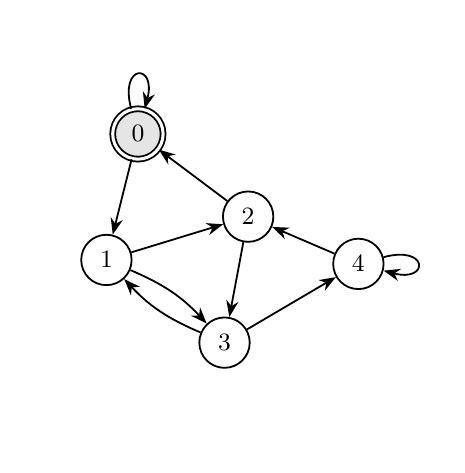
\begin{tikzpicture}[
  x=1cm,y=1cm,>=Stealth,
  f1m5 vertex/.style={circle,draw=black,line width=.65pt,minimum size=6.4mm,inner sep=0pt,font=\small},
  f1m5 root/.style={f1m5 vertex,double,double distance=1.1pt},
  f1m5 port zero/.style={->,draw=black,line width=.65pt},
  f1m5 port one/.style={->,draw=black,line width=.65pt},
  f1m5 label/.style={font=\scriptsize,fill=white,inner sep=1.1pt}
]
\path[use as bounding box] (-2.60,-2.65) rectangle (2.60,2.65);
\node[f1m5 root,fill=black!10] (q0) at (-1.20,1.30) {$ 0 $};
\node[f1m5 vertex] (q1) at (-1.60,-0.30) {$ 1 $};
\node[f1m5 vertex] (q2) at (0.20,0.25) {$ 2 $};
\node[f1m5 vertex] (q3) at (-0.10,-1.35) {$ 3 $};
\node[f1m5 vertex] (q4) at (1.60,-0.35) {$ 4 $};
% edge 0 0 0
\draw[f1m5 port zero] (q0) edge[loop above,min distance=6mm] (q0);
% edge 0 1 1
\draw[f1m5 port one] (q0) edge[] (q1);
% edge 1 0 2
\draw[f1m5 port zero] (q1) edge[] (q2);
% edge 1 1 3
\draw[f1m5 port one] (q1) edge[bend left=12] (q3);
% edge 2 0 0
\draw[f1m5 port zero] (q2) edge[] (q0);
% edge 2 1 3
\draw[f1m5 port one] (q2) edge[] (q3);
% edge 3 0 1
\draw[f1m5 port zero] (q3) edge[bend left=12] (q1);
% edge 3 1 4
\draw[f1m5 port one] (q3) edge[] (q4);
% edge 4 0 2
\draw[f1m5 port zero] (q4) edge[] (q2);
% edge 4 1 4
\draw[f1m5 port one] (q4) edge[loop right,min distance=6mm] (q4);
\end{tikzpicture}
}\par
\small\textbf{(c)} $H=15$. Optimal starts: $\{0\}$.\\1 distinct rooted maximizing class.\par\end{minipage}
\hfill
\begin{minipage}[t]{.48\textwidth}\centering
\resizebox{6.9cm}{!}{% Five-state extremal seed graph (d).
% Requires \usepackage{tikz} and \usetikzlibrary{arrows.meta}.
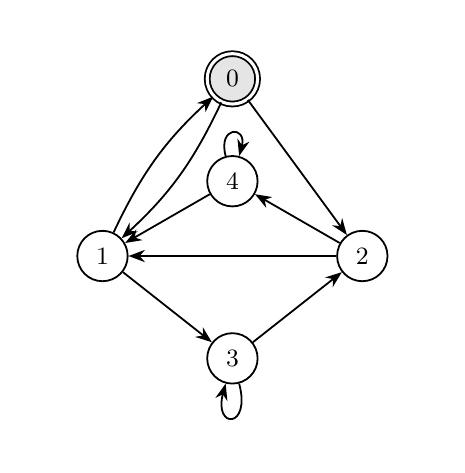
\begin{tikzpicture}[
  x=1cm,y=1cm,>=Stealth,
  f1m5 vertex/.style={circle,draw=black,line width=.65pt,minimum size=6.4mm,inner sep=0pt,font=\small},
  f1m5 root/.style={f1m5 vertex,double,double distance=1.1pt},
  f1m5 port zero/.style={->,draw=black,line width=.65pt},
  f1m5 port one/.style={->,draw=black,line width=.65pt},
  f1m5 label/.style={font=\scriptsize,fill=white,inner sep=1.1pt}
]
\path[use as bounding box] (-2.60,-2.65) rectangle (2.60,2.65);
\node[f1m5 root,fill=black!10] (q0) at (0.00,2.00) {$ 0 $};
\node[f1m5 vertex] (q1) at (-1.65,-0.25) {$ 1 $};
\node[f1m5 vertex] (q2) at (1.65,-0.25) {$ 2 $};
\node[f1m5 vertex] (q3) at (0.00,-1.55) {$ 3 $};
\node[f1m5 vertex] (q4) at (0.00,0.70) {$ 4 $};
% edge 0 0 1
\draw[f1m5 port zero] (q0) edge[bend left=11] (q1);
% edge 0 1 2
\draw[f1m5 port one] (q0) edge[] (q2);
% edge 1 0 0
\draw[f1m5 port zero] (q1) edge[bend left=11] (q0);
% edge 1 1 3
\draw[f1m5 port one] (q1) edge[] (q3);
% edge 2 0 1
\draw[f1m5 port zero] (q2) edge[] (q1);
% edge 2 1 4
\draw[f1m5 port one] (q2) edge[] (q4);
% edge 3 0 2
\draw[f1m5 port zero] (q3) edge[] (q2);
% edge 3 1 3
\draw[f1m5 port one] (q3) edge[loop below,min distance=6mm] (q3);
% edge 4 0 1
\draw[f1m5 port zero] (q4) edge[] (q1);
% edge 4 1 4
\draw[f1m5 port one] (q4) edge[loop above,min distance=4mm] (q4);
\end{tikzpicture}
}\par
\small\textbf{(d)} $H=15$. Optimal starts: $\{0\}$.\\1 distinct rooted maximizing class.\par\end{minipage}
\par\vspace{5mm}
\clearpage
{\LARGE\bfseries $m=6$}\par\vspace{3mm}
Global maximum $F(6)=23$; all 2 rooted maximizing classes, grouped into 1 ordinary shape.\par\vspace{2mm}
Double-circled vertices are all optimal starting states. Choose one marked start at a time; each choice defines a separate rooted graph.\par\vspace{3mm}
\begin{minipage}[t]{.94\textwidth}\centering
\resizebox{10.3cm}{!}{% Family 1 rooted seed, m=6; key=000102030304020500010405.
% Requires \usepackage{tikz} and \usetikzlibrary{arrows.meta}.
% Score and global-maximality metadata belong in the surrounding caption.
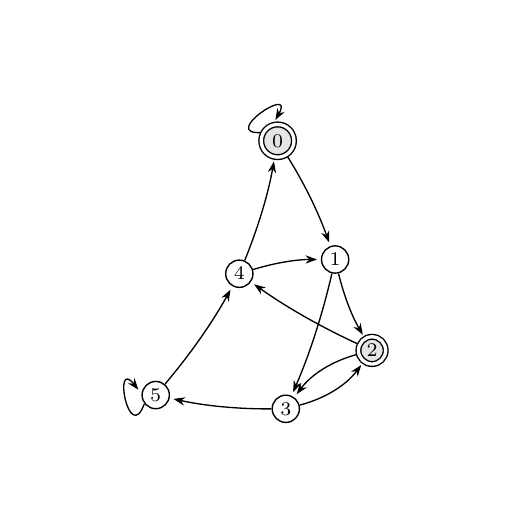
\begin{tikzpicture}[x=1cm,y=1cm,
  f1atlas state/.style={circle,draw=black,fill=white,line width=.5pt,inner sep=0pt,font=\fontsize{7}{8}\selectfont},
  f1atlas root/.style={f1atlas state,double,double distance=.42mm},
  f1atlas port0/.style={-{Stealth[length=1.45mm,width=1.05mm]},draw=black,line width=.48pt},
  f1atlas port1/.style={f1atlas port0},
  f1atlas label/.style={font=\fontsize{6}{7}\selectfont,fill=white,inner sep=.4pt}
]
\path[use as bounding box] (-3,-3) rectangle (3,3);
% edge 0 0 0
\draw[f1atlas port0] (-0.01801,1.66890) .. controls (-0.58479,1.62565) and (0.40721,2.28848) .. (0.14532,1.82727);
% edge 0 1 1
\draw[f1atlas port1] (0.29083,1.37783) .. controls (0.51198,1.02584) and (0.69086,0.65762) .. (0.82748,0.27317);
% edge 1 0 2
\draw[f1atlas port0] (0.94841,-0.12366) .. controls (1.01860,-0.41206) and (1.12128,-0.67085) .. (1.25645,-0.90002);
% edge 1 1 3
\draw[f1atlas port1] (0.86323,-0.12416) .. controls (0.74053,-0.65558) and (0.57631,-1.15715) .. (0.37056,-1.62886);
% edge 2 0 3
\draw[f1atlas port0] (1.19525,-1.14615) .. controls (0.86283,-1.23438) and (0.60312,-1.40409) .. (0.41611,-1.65528);
% edge 2 1 4
\draw[f1atlas port1] (1.20582,-1.02195) .. controls (0.72503,-0.80187) and (0.28175,-0.54748) .. (-0.12402,-0.25879);
% edge 3 0 2
\draw[f1atlas port0] (0.45674,-1.79302) .. controls (0.78916,-1.70479) and (1.04887,-1.53508) .. (1.23588,-1.28389);
% edge 3 1 5
\draw[f1atlas port1] (0.09369,-1.84138) .. controls (-0.34037,-1.84371) and (-0.75436,-1.80166) .. (-1.14828,-1.71522);
% edge 4 0 0
\draw[f1atlas port0] (-0.24271,0.04609) .. controls (-0.06772,0.47782) and (0.05578,0.89651) .. (0.12781,1.30216);
% edge 4 1 1
\draw[f1atlas port1] (-0.13549,-0.07108) .. controls (0.14336,0.01408) and (0.41319,0.05647) .. (0.67399,0.05607);
% edge 5 0 4
\draw[f1atlas port0] (-1.25452,-1.52477) .. controls (-0.92941,-1.14010) and (-0.65247,-0.74083) .. (-0.42370,-0.32697);
% edge 5 1 5
\draw[f1atlas port1] (-1.51939,-1.77913) .. controls (-1.71554,-2.30729) and (-1.92077,-1.18710) .. (-1.59423,-1.59784);
% state 0
\node[f1atlas root,minimum size=4.1538mm,fill=black!10] (q0) at (0.17420,1.56346) {$ 0 $};
% state 1
\node[f1atlas state,minimum size=3.4615mm] (q1) at (0.90476,0.05572) {$ 1 $};
% state 2
\node[f1atlas root,minimum size=3.4615mm,fill=black!10] (q2) at (1.37369,-1.09879) {$ 2 $};
% state 3
\node[f1atlas state,minimum size=3.4615mm] (q3) at (0.27830,-1.84038) {$ 3 $};
% state 4
\node[f1atlas state,minimum size=3.4615mm] (q4) at (-0.31206,-0.12501) {$ 4 $};
% state 5
\node[f1atlas state,minimum size=3.4615mm] (q5) at (-1.37369,-1.66577) {$ 5 $};
\end{tikzpicture}
}\par
\small\textbf{(a)} $H=23$. Optimal starts: $\{0, 2\}$.\\2 distinct rooted maximizing classes.\par\end{minipage}
\clearpage
{\LARGE\bfseries $m=7$}\par\vspace{3mm}
Global maximum $F(7)=34$; all 8 rooted maximizing classes, grouped into 4 ordinary shapes.\par\vspace{2mm}
Double-circled vertices are all optimal starting states. Choose one marked start at a time; each choice defines a separate rooted graph.\par\vspace{3mm}
\begin{minipage}[t]{.48\textwidth}\centering
\resizebox{6.9cm}{!}{% Family 1 rooted seed, m=7; key=0102000304050106000304050206.
% Requires \usepackage{tikz} and \usetikzlibrary{arrows.meta}.
% Score and global-maximality metadata belong in the surrounding caption.
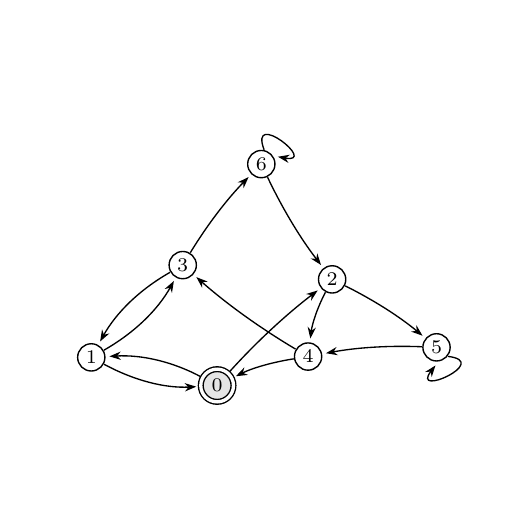
\begin{tikzpicture}[x=1cm,y=1cm,
  f1atlas state/.style={circle,draw=black,fill=white,line width=.5pt,inner sep=0pt,font=\fontsize{7}{8}\selectfont},
  f1atlas root/.style={f1atlas state,double,double distance=.42mm},
  f1atlas port0/.style={-{Stealth[length=1.45mm,width=1.05mm]},draw=black,line width=.48pt},
  f1atlas port1/.style={f1atlas port0},
  f1atlas label/.style={font=\fontsize{6}{7}\selectfont,fill=white,inner sep=.4pt}
]
\path[use as bounding box] (-3,-3) rectangle (3,3);
% edge 0 0 1
\draw[f1atlas port0] (-0.78696,-1.44041) .. controls (-1.15753,-1.24056) and (-1.54917,-1.15196) .. (-1.96188,-1.17459);
% edge 0 1 2
\draw[f1atlas port1] (-0.44732,-1.38154) .. controls (-0.09993,-0.99568) and (0.27697,-0.64744) .. (0.68338,-0.33684);
% edge 1 0 0
\draw[f1atlas port0] (-2.02982,-1.27486) .. controls (-1.63893,-1.48566) and (-1.24866,-1.58038) .. (-0.85899,-1.55901);
% edge 1 1 3
\draw[f1atlas port1] (-2.03183,-1.09597) .. controls (-1.64235,-0.87448) and (-1.34607,-0.58146) .. (-1.14301,-0.21692);
% edge 2 0 4
\draw[f1atlas port0] (0.78148,-0.36046) .. controls (0.67775,-0.55969) and (0.61389,-0.75549) .. (0.58988,-0.94785);
% edge 2 1 5
\draw[f1atlas port1] (1.03207,-0.27883) .. controls (1.39728,-0.46022) and (1.72487,-0.67140) .. (2.01482,-0.91236);
% edge 3 0 1
\draw[f1atlas port0] (-1.19118,-0.10658) .. controls (-1.58066,-0.32807) and (-1.87694,-0.62109) .. (-2.08001,-0.98563);
% edge 3 1 6
\draw[f1atlas port1] (-0.93452,0.14226) .. controls (-0.71457,0.50261) and (-0.46777,0.82271) .. (-0.19412,1.10256);
% edge 4 0 0
\draw[f1atlas port0] (0.37896,-1.20570) .. controls (0.09676,-1.25036) and (-0.14826,-1.32408) .. (-0.35611,-1.42685);
% edge 4 1 3
\draw[f1atlas port1] (0.40267,-1.08241) .. controls (-0.05851,-0.80790) and (-0.47866,-0.50314) .. (-0.85778,-0.16813);
% edge 5 0 4
\draw[f1atlas port0] (2.00785,-1.05231) .. controls (1.58275,-1.03495) and (1.17620,-1.06239) .. (0.78818,-1.13461);
% edge 5 1 5
\draw[f1atlas port1] (2.33698,-1.17454) .. controls (2.89658,-1.23991) and (1.85694,-1.70479) .. (2.17858,-1.29021);
% edge 6 0 2
\draw[f1atlas port0] (0.04650,1.10082) .. controls (0.24105,0.69168) and (0.46742,0.32004) .. (0.72562,-0.01410);
% edge 6 1 6
\draw[f1atlas port1] (0.00284,1.44870) .. controls (-0.19556,1.97601) and (0.69414,1.26511) .. (0.17825,1.36094);
% state 0
\node[f1atlas root,minimum size=4.1538mm,fill=black!10] (q0) at (-0.59400,-1.54447) {$ 0 $};
% state 1
\node[f1atlas state,minimum size=3.4615mm] (q1) at (-2.19231,-1.18723) {$ 1 $};
% state 2
\node[f1atlas state,minimum size=3.4615mm] (q2) at (0.86673,-0.19670) {$ 2 $};
% state 3
\node[f1atlas state,minimum size=3.4615mm] (q3) at (-1.03070,-0.01532) {$ 3 $};
% state 4
\node[f1atlas state,minimum size=3.4615mm] (q4) at (0.56131,-1.17684) {$ 4 $};
% state 5
\node[f1atlas state,minimum size=3.4615mm] (q5) at (2.19231,-1.05985) {$ 5 $};
% state 6
\node[f1atlas state,minimum size=3.4615mm] (q6) at (-0.03278,1.26755) {$ 6 $};
\end{tikzpicture}
}\par
\small\textbf{(a)} $H=34$. Optimal starts: $\{0\}$.\\1 distinct rooted maximizing class.\par\end{minipage}
\hfill
\begin{minipage}[t]{.48\textwidth}\centering
\resizebox{6.9cm}{!}{% Family 1 rooted seed, m=7; key=0001020302030405000604060105.
% Requires \usepackage{tikz} and \usetikzlibrary{arrows.meta}.
% Score and global-maximality metadata belong in the surrounding caption.
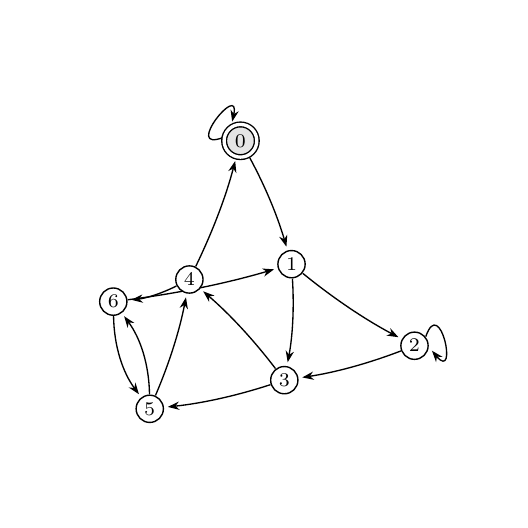
\begin{tikzpicture}[x=1cm,y=1cm,
  f1atlas state/.style={circle,draw=black,fill=white,line width=.5pt,inner sep=0pt,font=\fontsize{7}{8}\selectfont},
  f1atlas root/.style={f1atlas state,double,double distance=.42mm},
  f1atlas port0/.style={-{Stealth[length=1.45mm,width=1.05mm]},draw=black,line width=.48pt},
  f1atlas port1/.style={f1atlas port0},
  f1atlas label/.style={font=\fontsize{6}{7}\selectfont,fill=white,inner sep=.4pt}
]
\path[use as bounding box] (-3,-3) rectangle (3,3);
% edge 0 0 0
\draw[f1atlas port0] (-0.51231,1.60760) .. controls (-1.04120,1.39929) and (-0.28849,2.32495) .. (-0.40288,1.80705);
% edge 0 1 1
\draw[f1atlas port1] (-0.19230,1.37116) .. controls (0.01056,1.00058) and (0.17009,0.61621) .. (0.28630,0.21804);
% edge 1 0 2
\draw[f1atlas port0] (0.49406,-0.12012) .. controls (0.88520,-0.43894) and (1.29010,-0.70933) .. (1.70875,-0.93128);
% edge 1 1 3
\draw[f1atlas port1] (0.36244,-0.18774) .. controls (0.38562,-0.55973) and (0.36549,-0.91373) .. (0.30203,-1.24974);
% edge 2 0 2
\draw[f1atlas port0] (2.05593,-0.92297) .. controls (2.24093,-0.39081) and (2.46965,-1.50644) .. (2.13456,-1.10266);
% edge 2 1 3
\draw[f1atlas port1] (1.74024,-1.10545) .. controls (1.31976,-1.26660) and (0.90213,-1.37872) .. (0.48736,-1.44180);
% edge 3 0 4
\draw[f1atlas port0] (0.14730,-1.32967) .. controls (-0.13508,-0.95919) and (-0.44121,-0.63213) .. (-0.77109,-0.34850);
% edge 3 1 5
\draw[f1atlas port1] (0.08369,-1.53372) .. controls (-0.35605,-1.67706) and (-0.79061,-1.77125) .. (-1.21999,-1.81630);
% edge 4 0 0
\draw[f1atlas port0] (-0.86564,-0.03187) .. controls (-0.64534,0.42325) and (-0.47828,0.86942) .. (-0.36444,1.30664);
% edge 4 1 6
\draw[f1atlas port1] (-1.11113,-0.28074) .. controls (-1.30609,-0.37841) and (-1.49673,-0.43675) .. (-1.68305,-0.45575);
% edge 5 0 4
\draw[f1atlas port0] (-1.37684,-1.67067) .. controls (-1.19863,-1.25440) and (-1.06960,-0.83906) .. (-0.98974,-0.42465);
% edge 5 1 6
\draw[f1atlas port1] (-1.45270,-1.65580) .. controls (-1.45929,-1.27556) and (-1.56676,-0.94512) .. (-1.77509,-0.66447);
% edge 6 0 1
\draw[f1atlas port0] (-1.72952,-0.45570) .. controls (-1.08441,-0.37301) and (-0.46470,-0.24403) .. (0.12961,-0.06876);
% edge 6 1 5
\draw[f1atlas port1] (-1.90943,-0.66376) .. controls (-1.90283,-1.04399) and (-1.79537,-1.37443) .. (-1.58704,-1.65509);
% state 0
\node[f1atlas root,minimum size=4.1538mm,fill=black!10] (q0) at (-0.29757,1.56346) {$ 0 $};
% state 1
\node[f1atlas state,minimum size=3.4615mm] (q1) at (0.35096,-0.00348) {$ 1 $};
% state 2
\node[f1atlas state,minimum size=3.4615mm] (q2) at (1.91263,-1.03938) {$ 2 $};
% state 3
\node[f1atlas state,minimum size=3.4615mm] (q3) at (0.25921,-1.47650) {$ 3 $};
% state 4
\node[f1atlas state,minimum size=3.4615mm] (q4) at (-0.94607,-0.19805) {$ 4 $};
% state 5
\node[f1atlas state,minimum size=3.4615mm] (q5) at (-1.44949,-1.84038) {$ 5 $};
% state 6
\node[f1atlas state,minimum size=3.4615mm] (q6) at (-1.91263,-0.47917) {$ 6 $};
\end{tikzpicture}
}\par
\small\textbf{(b)} $H=34$. Optimal starts: $\{0\}$.\\1 distinct rooted maximizing class.\par\end{minipage}
\par\vspace{5mm}
\begin{minipage}[t]{.48\textwidth}\centering
\resizebox{6.9cm}{!}{% Family 1 rooted seed, m=7; key=0102010203040005030604060005.
% Requires \usepackage{tikz} and \usetikzlibrary{arrows.meta}.
% Score and global-maximality metadata belong in the surrounding caption.
\begin{tikzpicture}[x=1cm,y=1cm,
  f1atlas state/.style={circle,draw=black,fill=white,line width=.5pt,inner sep=0pt,font=\fontsize{7}{8}\selectfont},
  f1atlas root/.style={f1atlas state,double,double distance=.42mm},
  f1atlas port0/.style={-{Stealth[length=1.45mm,width=1.05mm]},draw=black,line width=.48pt},
  f1atlas port1/.style={f1atlas port0},
  f1atlas label/.style={font=\fontsize{6}{7}\selectfont,fill=white,inner sep=.4pt}
]
\path[use as bounding box] (-3,-3) rectangle (3,3);
% edge 0 0 1
\draw[f1atlas port0] (-0.32190,0.57857) .. controls (-0.17302,0.82020) and (-0.06244,1.07426) .. (0.00987,1.34074);
% edge 0 1 2
\draw[f1atlas port1] (-0.22222,0.43639) .. controls (-0.01648,0.47900) and (0.18657,0.48589) .. (0.38692,0.45706);
% edge 1 0 1
\draw[f1atlas port0] (-0.09707,1.64138) .. controls (-0.65654,1.57489) and (0.24657,2.26869) .. (0.03010,1.79070);
% edge 1 1 2
\draw[f1atlas port1] (0.17322,1.41020) .. controls (0.34180,1.15917) and (0.46636,0.90396) .. (0.54691,0.64457);
% edge 2 0 3
\draw[f1atlas port0] (0.51236,0.27095) .. controls (0.38793,0.08579) and (0.30338,-0.10033) .. (0.25874,-0.28740);
% edge 2 1 4
\draw[f1atlas port1] (0.64364,0.24175) .. controls (0.70112,-0.12887) and (0.71374,-0.48556) .. (0.68148,-0.82833);
% edge 3 0 0
\draw[f1atlas port0] (0.12442,-0.34585) .. controls (0.01440,-0.11963) and (-0.11032,0.06357) .. (-0.24975,0.20375);
% edge 3 1 5
\draw[f1atlas port1] (0.20738,-0.69647) .. controls (0.21130,-1.02392) and (0.17482,-1.33092) .. (0.09796,-1.61749);
% edge 4 0 3
\draw[f1atlas port0] (0.58121,-0.89106) .. controls (0.52938,-0.78097) and (0.46652,-0.69942) .. (0.39266,-0.64641);
% edge 4 1 6
\draw[f1atlas port1] (0.47682,-1.08213) .. controls (0.15843,-1.12397) and (-0.14438,-1.12357) .. (-0.43159,-1.08095);
% edge 5 0 4
\draw[f1atlas port0] (0.17738,-1.71912) .. controls (0.33998,-1.57748) and (0.46469,-1.42505) .. (0.55150,-1.26183);
% edge 5 1 6
\draw[f1atlas port1] (-0.01811,-1.66456) .. controls (-0.09776,-1.41571) and (-0.24200,-1.24246) .. (-0.45082,-1.14482);
% edge 6 0 0
\draw[f1atlas port0] (-0.60887,-0.86964) .. controls (-0.50773,-0.51769) and (-0.45284,-0.18560) .. (-0.44422,0.12663);
% edge 6 1 5
\draw[f1atlas port1] (-0.60358,-1.22290) .. controls (-0.52392,-1.47175) and (-0.37969,-1.64499) .. (-0.17087,-1.74263);
% state 0
\node[f1atlas root,minimum size=4.1538mm,fill=black!10] (q0) at (-0.43689,0.39192) {$ 0 $};
% state 1
\node[f1atlas state,minimum size=3.4615mm] (q1) at (0.07030,1.56346) {$ 1 $};
% state 2
\node[f1atlas state,minimum size=3.4615mm] (q2) at (0.61534,0.42418) {$ 2 $};
% state 3
\node[f1atlas state,minimum size=3.4615mm] (q3) at (0.20517,-0.51187) {$ 3 $};
% state 4
\node[f1atlas state,minimum size=3.4615mm] (q4) at (0.65986,-1.05808) {$ 4 $};
% state 5
\node[f1atlas state,minimum size=3.4615mm] (q5) at (0.03817,-1.84038) {$ 5 $};
% state 6
\node[f1atlas state,minimum size=3.4615mm] (q6) at (-0.65986,-1.04707) {$ 6 $};
\end{tikzpicture}
}\par
\small\textbf{(c)} $H=34$. Optimal starts: $\{0\}$.\\1 distinct rooted maximizing class.\par\end{minipage}
\hfill
\begin{minipage}[t]{.48\textwidth}\centering
\resizebox{6.9cm}{!}{% Family 1 rooted seed, m=7; key=0001020304050406050600010203.
% Requires \usepackage{tikz} and \usetikzlibrary{arrows.meta}.
% Score and global-maximality metadata belong in the surrounding caption.
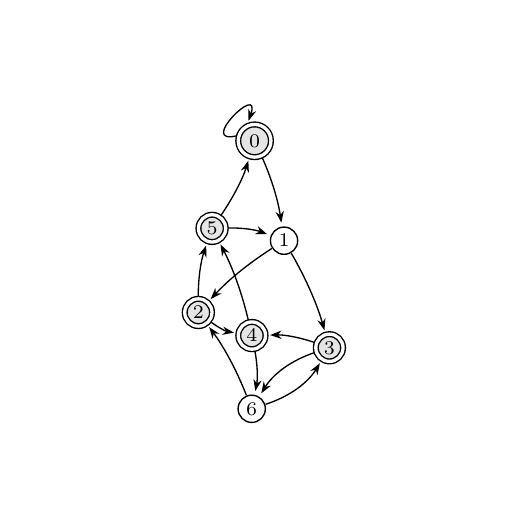
\begin{tikzpicture}[x=1cm,y=1cm,
  f1atlas state/.style={circle,draw=black,fill=white,line width=.5pt,inner sep=0pt,font=\fontsize{7}{8}\selectfont},
  f1atlas root/.style={f1atlas state,double,double distance=.42mm},
  f1atlas port0/.style={-{Stealth[length=1.45mm,width=1.05mm]},draw=black,line width=.48pt},
  f1atlas port1/.style={f1atlas port0},
  f1atlas label/.style={font=\fontsize{6}{7}\selectfont,fill=white,inner sep=.4pt}
]
\path[use as bounding box] (-3,-3) rectangle (3,3);
% edge 0 0 0
\draw[f1atlas port0] (-0.32653,1.63146) .. controls (-0.87549,1.48394) and (-0.02348,2.31910) .. (-0.19538,1.81735);
% edge 0 1 1
\draw[f1atlas port1] (-0.02764,1.36377) .. controls (0.09579,1.09134) and (0.17901,0.81101) .. (0.22201,0.52280);
% edge 1 0 2
\draw[f1atlas port0] (0.10042,0.19525) .. controls (-0.19812,0.00476) and (-0.45692,-0.20942) .. (-0.67597,-0.44730);
% edge 1 1 3
\draw[f1atlas port1] (0.34862,0.13482) .. controls (0.53565,-0.18793) and (0.67588,-0.51394) .. (0.76930,-0.84321);
% edge 2 0 4
\draw[f1atlas port0] (-0.68546,-0.72896) .. controls (-0.58104,-0.80855) and (-0.47922,-0.85649) .. (-0.38002,-0.87276);
% edge 2 1 5
\draw[f1atlas port1] (-0.83363,-0.43244) .. controls (-0.83538,-0.18958) and (-0.80182,0.03214) .. (-0.73295,0.23274);
% edge 3 0 4
\draw[f1atlas port0] (0.65821,-1.00375) .. controls (0.45565,-0.93224) and (0.26238,-0.89895) .. (0.07840,-0.90390);
% edge 3 1 6
\draw[f1atlas port1] (0.65667,-1.12214) .. controls (0.34980,-1.22160) and (0.11979,-1.39553) .. (-0.03336,-1.64395);
% edge 4 0 5
\draw[f1atlas port0] (-0.19425,-0.73032) .. controls (-0.27716,-0.37504) and (-0.39608,-0.04942) .. (-0.55099,0.24655);
% edge 4 1 6
\draw[f1atlas port1] (-0.11678,-1.09128) .. controls (-0.07964,-1.28073) and (-0.07705,-1.45502) .. (-0.10901,-1.61414);
% edge 5 0 0
\draw[f1atlas port0] (-0.55376,0.60337) .. controls (-0.38793,0.84575) and (-0.26917,1.08136) .. (-0.19746,1.31022);
% edge 5 1 1
\draw[f1atlas port1] (-0.47346,0.45599) .. controls (-0.28142,0.46118) and (-0.11008,0.43490) .. (0.04057,0.37715);
% edge 6 0 2
\draw[f1atlas port0] (-0.22204,-1.66858) .. controls (-0.34910,-1.34551) and (-0.50676,-1.05683) .. (-0.69499,-0.80253);
% edge 6 1 3
\draw[f1atlas port1] (0.02116,-1.78346) .. controls (0.32804,-1.68400) and (0.55805,-1.51006) .. (0.71119,-1.26165);
% state 0
\node[f1atlas root,minimum size=4.1538mm,fill=black!10] (q0) at (-0.11812,1.56346) {$ 0 $};
% state 1
\node[f1atlas state,minimum size=3.4615mm] (q1) at (0.25606,0.29456) {$ 1 $};
% state 2
\node[f1atlas root,minimum size=3.4615mm,fill=black!10] (q2) at (-0.83229,-0.61705) {$ 2 $};
% state 3
\node[f1atlas root,minimum size=3.4615mm,fill=black!10] (q3) at (0.83229,-1.06521) {$ 3 $};
% state 4
\node[f1atlas root,minimum size=3.4615mm,fill=black!10] (q4) at (-0.15229,-0.91011) {$ 4 $};
% state 5
\node[f1atlas root,minimum size=3.4615mm,fill=black!10] (q5) at (-0.65801,0.45101) {$ 5 $};
% state 6
\node[f1atlas state,minimum size=3.4615mm] (q6) at (-0.15446,-1.84038) {$ 6 $};
\end{tikzpicture}
}\par
\small\textbf{(d)} $H=34$. Optimal starts: $\{0, 2, 3, 4, 5\}$.\\5 distinct rooted maximizing classes.\par\end{minipage}
\par\vspace{5mm}
\clearpage
{\LARGE\bfseries $m=8$}\par\vspace{3mm}
\textbf{One candidate found.} The working estimate is $49$ (rough range $48$--$50$), with a verified pair of length $50$. The marked start $0$ gives the best current estimate; start $2$ of the same graph is the runner-up.\par\vspace{2mm}
All eight starting states of this graph were checked heuristically. The returned pair lengths are:\par\smallskip\begin{center}\begin{tabular}{r|rrrrrrrr}Start &0&1&2&3&4&5&6&7\\\hline Pair length &50&42&49&39&43&47&43&46\end{tabular}\end{center}\vspace{2mm}
\begin{minipage}[t]{.94\textwidth}\centering
\resizebox{10.3cm}{!}{% Family 1 rooted seed, m=8; key=01020003040501060003020705060407.
% Requires \usepackage{tikz} and \usetikzlibrary{arrows.meta}.
% Score and global-maximality metadata belong in the surrounding caption.
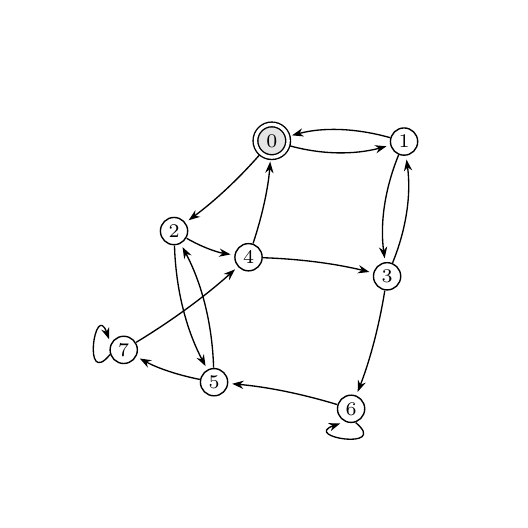
\begin{tikzpicture}[x=1cm,y=1cm,
  f1atlas state/.style={circle,draw=black,fill=white,line width=.5pt,inner sep=0pt,font=\fontsize{7}{8}\selectfont},
  f1atlas root/.style={f1atlas state,double,double distance=.42mm},
  f1atlas port0/.style={-{Stealth[length=1.45mm,width=1.05mm]},draw=black,line width=.48pt},
  f1atlas port1/.style={f1atlas port0},
  f1atlas label/.style={font=\fontsize{6}{7}\selectfont,fill=white,inner sep=.4pt}
]
\path[use as bounding box] (-3,-3) rectangle (3,3);
% edge 0 0 1
\draw[f1atlas port0] (0.31147,1.50412) .. controls (0.72976,1.38652) and (1.14503,1.38303) .. (1.55726,1.49367);
% edge 0 1 2
\draw[f1atlas port1] (-0.04354,1.39812) .. controls (-0.31969,1.08096) and (-0.62372,0.79963) .. (-0.95565,0.55415);
% edge 1 0 0
\draw[f1atlas port0] (1.60242,1.60346) .. controls (1.16191,1.72732) and (0.74668,1.73691) .. (0.35673,1.63225);
% edge 1 1 3
\draw[f1atlas port1] (1.71052,1.38251) .. controls (1.53250,0.94535) and (1.47347,0.50819) .. (1.53342,0.07104);
% edge 2 0 4
\draw[f1atlas port0] (-0.98097,0.32519) .. controls (-0.79286,0.21749) and (-0.60694,0.14921) .. (-0.42320,0.12035);
% edge 2 1 5
\draw[f1atlas port1] (-1.13557,0.23239) .. controls (-1.11864,-0.32373) and (-0.98713,-0.83402) .. (-0.74104,-1.29846);
% edge 3 0 1
\draw[f1atlas port0] (1.63440,0.01339) .. controls (1.81242,0.45055) and (1.87145,0.88771) .. (1.81150,1.32486);
% edge 3 1 6
\draw[f1atlas port1] (1.53540,-0.33986) .. controls (1.46196,-0.79541) and (1.34722,-1.22389) .. (1.19118,-1.62530);
% edge 4 0 0
\draw[f1atlas port0] (-0.13731,0.25984) .. controls (-0.01703,0.62388) and (0.05554,0.97022) .. (0.08040,1.29883);
% edge 4 1 3
\draw[f1atlas port1] (-0.01071,0.07842) .. controls (0.46133,0.06275) and (0.91178,0.00239) .. (1.34064,-0.10268);
% edge 5 0 2
\draw[f1atlas port0] (-0.63861,-1.31785) .. controls (-0.65554,-0.76172) and (-0.78705,-0.25144) .. (-1.03314,0.21301);
% edge 5 1 7
\draw[f1atlas port1] (-0.81417,-1.46694) .. controls (-1.09650,-1.41171) and (-1.35076,-1.32320) .. (-1.57696,-1.20141);
% edge 6 0 5
\draw[f1atlas port0] (0.93095,-1.78661) .. controls (0.48024,-1.64938) and (0.03555,-1.56140) .. (-0.40312,-1.52267);
% edge 6 1 6
\draw[f1atlas port1] (1.16594,-2.01553) .. controls (1.59865,-2.37634) and (0.47405,-2.19687) .. (0.97007,-2.02572);
% edge 7 0 4
\draw[f1atlas port0] (-1.62230,-0.99624) .. controls (-1.16254,-0.71731) and (-0.74408,-0.40846) .. (-0.36691,-0.06967);
% edge 7 1 7
\draw[f1atlas port1] (-1.95478,-1.15187) .. controls (-2.31191,-1.58763) and (-2.14199,-0.46154) .. (-1.96664,-0.95609);
% state 0
\node[f1atlas root,minimum size=4.1538mm,fill=black!10] (q0) at (0.10042,1.56346) {$ 0 $};
% state 1
\node[f1atlas state,minimum size=3.4615mm] (q1) at (1.78014,1.55349) {$ 1 $};
% state 2
\node[f1atlas state,minimum size=3.4615mm] (q2) at (-1.14119,0.41692) {$ 2 $};
% state 3
\node[f1atlas state,minimum size=3.4615mm] (q3) at (1.56478,-0.15759) {$ 3 $};
% state 4
\node[f1atlas state,minimum size=3.4615mm] (q4) at (-0.19522,0.08454) {$ 4 $};
% state 5
\node[f1atlas state,minimum size=3.4615mm] (q5) at (-0.63299,-1.50238) {$ 5 $};
% state 6
\node[f1atlas state,minimum size=3.4615mm] (q6) at (1.10756,-1.84038) {$ 6 $};
% state 7
\node[f1atlas state,minimum size=3.4615mm] (q7) at (-1.78014,-1.09200) {$ 7 $};
\end{tikzpicture}
}\par
\small\textbf{(a)} Best current estimated start: $0$.\\Finder length $50$; working estimate $H\approx49$.\par\end{minipage}
\clearpage
{\LARGE\bfseries $m=9$}\par\vspace{3mm}
\textbf{Constructive lower-bound example.} The indicated start gives $H\ge34$ by a static-mask projection onto a certified seven-state maximizer. This graph has not been certified globally optimal; its exact score is unresolved.\par\vspace{3mm}
\begin{minipage}[t]{.94\textwidth}\centering
\resizebox{10.3cm}{!}{% Family 1 rooted seed, m=9; key=010202030405000204050607000806080207.
% Requires \usepackage{tikz} and \usetikzlibrary{arrows.meta}.
% Score and global-maximality metadata belong in the surrounding caption.
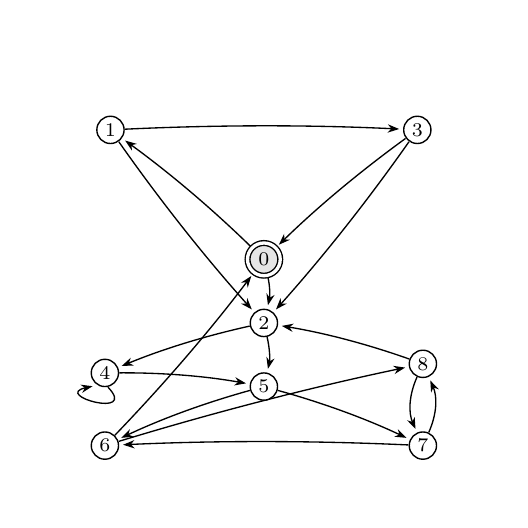
\begin{tikzpicture}[x=1cm,y=1cm,
  f1atlas state/.style={circle,draw=black,fill=white,line width=.5pt,inner sep=0pt,font=\fontsize{7}{8}\selectfont},
  f1atlas root/.style={f1atlas state,double,double distance=.42mm},
  f1atlas port0/.style={-{Stealth[length=1.45mm,width=1.05mm]},draw=black,line width=.48pt},
  f1atlas port1/.style={f1atlas port0},
  f1atlas label/.style={font=\fontsize{6}{7}\selectfont,fill=white,inner sep=.4pt}
]
\path[use as bounding box] (-3,-3) rectangle (3,3);
% edge 0 0 1
\draw[f1atlas port0] (-0.15690,0.21081) .. controls (-0.66213,0.70384) and (-1.19713,1.15565) .. (-1.76190,1.56623);
% edge 0 1 2
\draw[f1atlas port1] (0.04885,-0.15603) .. controls (0.07782,-0.28278) and (0.07868,-0.40578) .. (0.05142,-0.52503);
% edge 1 0 2
\draw[f1atlas port0] (-1.84240,1.55088) .. controls (-1.31183,0.79598) and (-0.74902,0.08632) .. (-0.15396,-0.57810);
% edge 1 1 3
\draw[f1atlas port1] (-1.76415,1.71066) .. controls (-0.58805,1.76637) and (0.57268,1.76710) .. (1.71805,1.71284);
% edge 2 0 4
\draw[f1atlas port0] (-0.18027,-0.78984) .. controls (-0.75162,-0.91611) and (-1.29350,-1.08502) .. (-1.80592,-1.29656);
% edge 2 1 5
\draw[f1atlas port1] (0.04114,-0.92997) .. controls (0.07525,-1.07922) and (0.07868,-1.21347) .. (0.05142,-1.33272);
% edge 3 0 0
\draw[f1atlas port0] (1.79923,1.59337) .. controls (1.20958,1.16469) and (0.67314,0.71458) .. (0.18993,0.24304);
% edge 3 1 2
\draw[f1atlas port1] (1.84240,1.55088) .. controls (1.31183,0.79598) and (0.74902,0.08632) .. (0.15396,-0.57810);
% edge 4 0 4
\draw[f1atlas port0] (-1.98070,-1.56516) .. controls (-1.59080,-1.97187) and (-2.68847,-1.66841) .. (-2.17649,-1.55351);
% edge 4 1 5
\draw[f1atlas port1] (-1.83462,-1.38363) .. controls (-1.27936,-1.38067) and (-0.74355,-1.42519) .. (-0.22719,-1.51721);
% edge 5 0 6
\draw[f1atlas port0] (-0.17792,-1.60696) .. controls (-0.75381,-1.76643) and (-1.29802,-1.96716) .. (-1.81055,-2.20916);
% edge 5 1 7
\draw[f1atlas port1] (0.17792,-1.60696) .. controls (0.75381,-1.76643) and (1.29802,-1.96716) .. (1.81055,-2.20916);
% edge 6 0 0
\draw[f1atlas port0] (-1.89126,-2.17463) .. controls (-1.25669,-1.51483) and (-0.67962,-0.84129) .. (-0.16004,-0.15401);
% edge 6 1 8
\draw[f1atlas port1] (-1.84264,-2.25385) .. controls (-0.62954,-1.88399) and (0.58248,-1.57163) .. (1.79341,-1.31676);
% edge 7 0 6
\draw[f1atlas port0] (1.83481,-2.29926) .. controls (0.61160,-2.24334) and (-0.59623,-2.24264) .. (-1.78870,-2.29715);
% edge 7 1 8
\draw[f1atlas port1] (2.09421,-2.13899) .. controls (2.19807,-1.90530) and (2.20432,-1.68568) .. (2.11296,-1.48011);
% edge 8 0 2
\draw[f1atlas port0] (1.84518,-1.20766) .. controls (1.30346,-1.01603) and (0.76430,-0.87599) .. (0.22770,-0.78753);
% edge 8 1 7
\draw[f1atlas port1] (1.94425,-1.43793) .. controls (1.84039,-1.67162) and (1.83414,-1.89125) .. (1.92551,-2.09681);
% state 0
\node[f1atlas root,minimum size=4.1538mm,fill=black!10] (q0) at (0.00000,0.05769) {$ 0 $};
% state 1
\node[f1atlas state,minimum size=3.4615mm] (q1) at (-1.94856,1.70192) {$ 1 $};
% state 2
\node[f1atlas state,minimum size=3.4615mm] (q2) at (0.00000,-0.75000) {$ 2 $};
% state 3
\node[f1atlas state,minimum size=3.4615mm] (q3) at (1.94856,1.70192) {$ 3 $};
% state 4
\node[f1atlas state,minimum size=3.4615mm] (q4) at (-2.01923,-1.38462) {$ 4 $};
% state 5
\node[f1atlas state,minimum size=3.4615mm] (q5) at (0.00000,-1.55769) {$ 5 $};
% state 6
\node[f1atlas state,minimum size=3.4615mm] (q6) at (-2.01923,-2.30769) {$ 6 $};
% state 7
\node[f1atlas state,minimum size=3.4615mm] (q7) at (2.01923,-2.30769) {$ 7 $};
% state 8
\node[f1atlas state,minimum size=3.4615mm] (q8) at (2.01923,-1.26923) {$ 8 $};
\end{tikzpicture}
}\par
\small\textbf{(a)} Example start: $0$. Proved $H\ge34$.\\Exact score and global maximum unresolved.\par\end{minipage}
\clearpage
{\LARGE\bfseries $m=10$}\par\vspace{3mm}
\textbf{Constructive lower-bound example.} The indicated start gives $H\ge34$ by a static-mask projection onto a certified seven-state maximizer. This graph has not been certified globally optimal; its exact score is unresolved.\par\vspace{3mm}
\begin{minipage}[t]{.94\textwidth}\centering
\resizebox{10.3cm}{!}{% Family 1 rooted seed, m=10; key=0102020304050206040507080002000907090208.
% Requires \usepackage{tikz} and \usetikzlibrary{arrows.meta}.
% Score and global-maximality metadata belong in the surrounding caption.
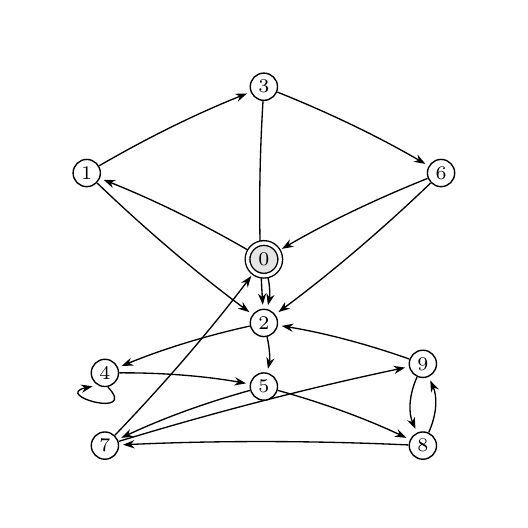
\begin{tikzpicture}[x=1cm,y=1cm,
  f1atlas state/.style={circle,draw=black,fill=white,line width=.5pt,inner sep=0pt,font=\fontsize{7}{8}\selectfont},
  f1atlas root/.style={f1atlas state,double,double distance=.42mm},
  f1atlas port0/.style={-{Stealth[length=1.45mm,width=1.05mm]},draw=black,line width=.48pt},
  f1atlas port1/.style={f1atlas port0},
  f1atlas label/.style={font=\fontsize{6}{7}\selectfont,fill=white,inner sep=.4pt}
]
\path[use as bounding box] (-3,-3) rectangle (3,3);
% edge 0 0 1
\draw[f1atlas port0] (-0.18949,0.16795) .. controls (-0.78621,0.51515) and (-1.40160,0.81527) .. (-2.03567,1.06831);
% edge 0 1 2
\draw[f1atlas port1] (0.04885,-0.15603) .. controls (0.07782,-0.28278) and (0.07868,-0.40578) .. (0.05142,-0.52503);
% edge 1 0 2
\draw[f1atlas port0] (-2.11680,1.02602) .. controls (-1.49535,0.42964) and (-0.85146,-0.11644) .. (-0.18514,-0.61224);
% edge 1 1 3
\draw[f1atlas port1] (-2.09043,1.24669) .. controls (-1.47376,1.60550) and (-0.84840,1.91143) .. (-0.21433,2.16447);
% edge 2 0 4
\draw[f1atlas port0] (-0.18027,-0.78984) .. controls (-0.75162,-0.91611) and (-1.29350,-1.08502) .. (-1.80592,-1.29656);
% edge 2 1 5
\draw[f1atlas port1] (0.04114,-0.92997) .. controls (0.07525,-1.07922) and (0.07868,-1.21347) .. (0.05142,-1.33272);
% edge 3 0 2
\draw[f1atlas port0] (-0.01134,2.06573) .. controls (-0.06532,1.18858) and (-0.06626,0.32678) .. (-0.01417,-0.51967);
% edge 3 1 6
\draw[f1atlas port1] (0.17147,2.18157) .. controls (0.83411,1.91713) and (1.46046,1.61324) .. (2.05054,1.26990);
% edge 4 0 4
\draw[f1atlas port0] (-1.98070,-1.56516) .. controls (-1.59080,-1.97187) and (-2.68847,-1.66841) .. (-2.17649,-1.55351);
% edge 4 1 5
\draw[f1atlas port1] (-1.83462,-1.38363) .. controls (-1.27936,-1.38067) and (-0.74355,-1.42519) .. (-0.22719,-1.51721);
% edge 5 0 7
\draw[f1atlas port0] (-0.17792,-1.60696) .. controls (-0.75381,-1.76643) and (-1.29802,-1.96716) .. (-1.81055,-2.20916);
% edge 5 1 8
\draw[f1atlas port1] (0.17792,-1.60696) .. controls (0.75381,-1.76643) and (1.29802,-1.96716) .. (1.81055,-2.20916);
% edge 6 0 0
\draw[f1atlas port0] (2.07853,1.08542) .. controls (1.41589,0.82097) and (0.79951,0.52289) .. (0.22938,0.19116);
% edge 6 1 2
\draw[f1atlas port1] (2.11680,1.02602) .. controls (1.49535,0.42964) and (0.85146,-0.11644) .. (0.18514,-0.61224);
% edge 7 0 0
\draw[f1atlas port0] (-1.89126,-2.17463) .. controls (-1.25669,-1.51483) and (-0.67962,-0.84129) .. (-0.16004,-0.15401);
% edge 7 1 9
\draw[f1atlas port1] (-1.84264,-2.25385) .. controls (-0.62954,-1.88399) and (0.58248,-1.57163) .. (1.79341,-1.31676);
% edge 8 0 7
\draw[f1atlas port0] (1.83481,-2.29926) .. controls (0.61160,-2.24334) and (-0.59623,-2.24264) .. (-1.78870,-2.29715);
% edge 8 1 9
\draw[f1atlas port1] (2.09421,-2.13899) .. controls (2.19807,-1.90530) and (2.20432,-1.68568) .. (2.11296,-1.48011);
% edge 9 0 2
\draw[f1atlas port0] (1.84518,-1.20766) .. controls (1.30346,-1.01603) and (0.76430,-0.87599) .. (0.22770,-0.78753);
% edge 9 1 8
\draw[f1atlas port1] (1.94425,-1.43793) .. controls (1.84039,-1.67162) and (1.83414,-1.89125) .. (1.92551,-2.09681);
% state 0
\node[f1atlas root,minimum size=4.1538mm,fill=black!10] (q0) at (0.00000,0.05769) {$ 0 $};
% state 1
\node[f1atlas state,minimum size=3.4615mm] (q1) at (-2.25000,1.15385) {$ 1 $};
% state 2
\node[f1atlas state,minimum size=3.4615mm] (q2) at (0.00000,-0.75000) {$ 2 $};
% state 3
\node[f1atlas state,minimum size=3.4615mm] (q3) at (-0.00000,2.25000) {$ 3 $};
% state 4
\node[f1atlas state,minimum size=3.4615mm] (q4) at (-2.01923,-1.38462) {$ 4 $};
% state 5
\node[f1atlas state,minimum size=3.4615mm] (q5) at (0.00000,-1.55769) {$ 5 $};
% state 6
\node[f1atlas state,minimum size=3.4615mm] (q6) at (2.25000,1.15385) {$ 6 $};
% state 7
\node[f1atlas state,minimum size=3.4615mm] (q7) at (-2.01923,-2.30769) {$ 7 $};
% state 8
\node[f1atlas state,minimum size=3.4615mm] (q8) at (2.01923,-2.30769) {$ 8 $};
% state 9
\node[f1atlas state,minimum size=3.4615mm] (q9) at (2.01923,-1.26923) {$ 9 $};
\end{tikzpicture}
}\par
\small\textbf{(a)} Example start: $0$. Proved $H\ge34$.\\Exact score and global maximum unresolved.\par\end{minipage}
\clearpage
{\LARGE\bfseries $m=11$}\par\vspace{3mm}
\textbf{Constructive lower-bound example.} The indicated start gives $H\ge34$ by a static-mask projection onto a certified seven-state maximizer. This graph has not been certified globally optimal; its exact score is unresolved.\par\vspace{3mm}
\begin{minipage}[t]{.94\textwidth}\centering
\resizebox{10.3cm}{!}{% Family 1 rooted seed, m=11; key=01020203040502060405070802090010071000020208.
% Requires \usepackage{tikz} and \usetikzlibrary{arrows.meta}.
% Score and global-maximality metadata belong in the surrounding caption.
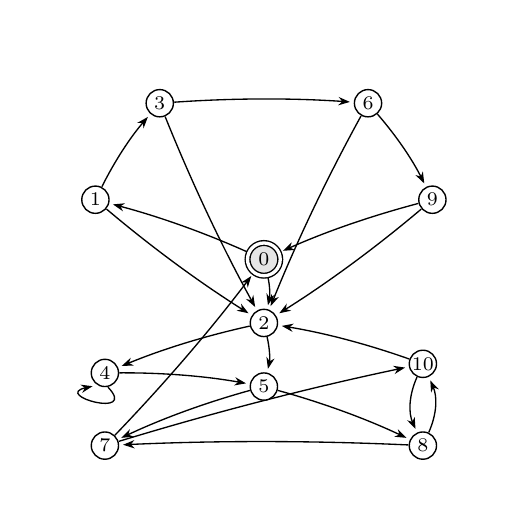
\begin{tikzpicture}[x=1cm,y=1cm,
  f1atlas state/.style={circle,draw=black,fill=white,line width=.5pt,inner sep=0pt,font=\fontsize{7}{8}\selectfont},
  f1atlas root/.style={f1atlas state,double,double distance=.42mm},
  f1atlas port0/.style={-{Stealth[length=1.45mm,width=1.05mm]},draw=black,line width=.48pt},
  f1atlas port1/.style={f1atlas port0},
  f1atlas label/.style={font=\fontsize{6}{7}\selectfont,fill=white,inner sep=.4pt}
]
\path[use as bounding box] (-3,-3) rectangle (3,3);
% edge 0 0 1
\draw[f1atlas port0] (-0.20006,0.14736) .. controls (-0.75944,0.39807) and (-1.33169,0.60095) .. (-1.91681,0.75600);
% edge 0 1 2
\draw[f1atlas port1] (0.04885,-0.15603) .. controls (0.07782,-0.28278) and (0.07868,-0.40578) .. (0.05142,-0.52503);
% edge 1 0 2
\draw[f1atlas port0] (-1.99880,0.69604) .. controls (-1.41589,0.20405) and (-0.81471,-0.23698) .. (-0.19528,-0.62703);
% edge 1 1 3
\draw[f1atlas port1] (-2.05734,0.98025) .. controls (-1.89111,1.31282) and (-1.69647,1.60809) .. (-1.47344,1.86608);
% edge 2 0 4
\draw[f1atlas port0] (-0.18027,-0.78984) .. controls (-0.75162,-0.91611) and (-1.29350,-1.08502) .. (-1.80592,-1.29656);
% edge 2 1 5
\draw[f1atlas port1] (0.04114,-0.92997) .. controls (0.07525,-1.07922) and (0.07868,-1.21347) .. (0.05142,-1.33272);
% edge 3 0 2
\draw[f1atlas port0] (-1.25355,1.86940) .. controls (-0.91430,1.02700) and (-0.53348,0.22129) .. (-0.11110,-0.54773);
% edge 3 1 6
\draw[f1atlas port1] (-1.13835,2.05351) .. controls (-0.37945,2.10648) and (0.36410,2.10755) .. (1.09231,2.05672);
% edge 4 0 4
\draw[f1atlas port0] (-1.98070,-1.56516) .. controls (-1.59080,-1.97187) and (-2.68847,-1.66841) .. (-2.17649,-1.55351);
% edge 4 1 5
\draw[f1atlas port1] (-1.83462,-1.38363) .. controls (-1.27936,-1.38067) and (-0.74355,-1.42519) .. (-0.22719,-1.51721);
% edge 5 0 7
\draw[f1atlas port0] (-0.17792,-1.60696) .. controls (-0.75381,-1.76643) and (-1.29802,-1.96716) .. (-1.81055,-2.20916);
% edge 5 1 8
\draw[f1atlas port1] (0.17792,-1.60696) .. controls (0.75381,-1.76643) and (1.29802,-1.96716) .. (1.81055,-2.20916);
% edge 6 0 2
\draw[f1atlas port0] (1.23364,1.87884) .. controls (0.79644,1.08285) and (0.41396,0.27793) .. (0.08621,-0.53594);
% edge 6 1 9
\draw[f1atlas port1] (1.44326,1.90099) .. controls (1.68641,1.61973) and (1.88423,1.32658) .. (2.03670,1.02154);
% edge 7 0 0
\draw[f1atlas port0] (-1.89126,-2.17463) .. controls (-1.25669,-1.51483) and (-0.67962,-0.84129) .. (-0.16004,-0.15401);
% edge 7 1 10
\draw[f1atlas port1] (-1.84264,-2.25385) .. controls (-0.62954,-1.88399) and (0.58248,-1.57163) .. (1.79341,-1.31676);
% edge 8 0 7
\draw[f1atlas port0] (1.83481,-2.29926) .. controls (0.61160,-2.24334) and (-0.59623,-2.24264) .. (-1.78870,-2.29715);
% edge 8 1 10
\draw[f1atlas port1] (2.09421,-2.13899) .. controls (2.19807,-1.90530) and (2.20432,-1.68568) .. (2.11296,-1.48011);
% edge 9 0 0
\draw[f1atlas port0] (1.96142,0.76783) .. controls (1.34657,0.60489) and (0.77348,0.40436) .. (0.24217,0.16623);
% edge 9 1 2
\draw[f1atlas port1] (1.99880,0.69604) .. controls (1.41589,0.20405) and (0.81471,-0.23698) .. (0.19528,-0.62703);
% edge 10 0 2
\draw[f1atlas port0] (1.84518,-1.20766) .. controls (1.30346,-1.01603) and (0.76430,-0.87599) .. (0.22770,-0.78753);
% edge 10 1 8
\draw[f1atlas port1] (1.94425,-1.43793) .. controls (1.84039,-1.67162) and (1.83414,-1.89125) .. (1.92551,-2.09681);
% state 0
\node[f1atlas root,minimum size=4.1538mm,fill=black!10] (q0) at (0.00000,0.05769) {$ 0 $};
% state 1
\node[f1atlas state,minimum size=3.4615mm] (q1) at (-2.13988,0.81512) {$ 1 $};
% state 2
\node[f1atlas state,minimum size=3.4615mm] (q2) at (0.00000,-0.75000) {$ 2 $};
% state 3
\node[f1atlas state,minimum size=3.4615mm] (q3) at (-1.32252,2.04065) {$ 3 $};
% state 4
\node[f1atlas state,minimum size=3.4615mm] (q4) at (-2.01923,-1.38462) {$ 4 $};
% state 5
\node[f1atlas state,minimum size=3.4615mm] (q5) at (0.00000,-1.55769) {$ 5 $};
% state 6
\node[f1atlas state,minimum size=3.4615mm] (q6) at (1.32252,2.04065) {$ 6 $};
% state 7
\node[f1atlas state,minimum size=3.4615mm] (q7) at (-2.01923,-2.30769) {$ 7 $};
% state 8
\node[f1atlas state,minimum size=3.4615mm] (q8) at (2.01923,-2.30769) {$ 8 $};
% state 9
\node[f1atlas state,minimum size=3.4615mm] (q9) at (2.13988,0.81512) {$ 9 $};
% state 10
\node[f1atlas state,minimum size=3.4615mm] (q10) at (2.01923,-1.26923) {$ 10 $};
\end{tikzpicture}
}\par
\small\textbf{(a)} Example start: $0$. Proved $H\ge34$.\\Exact score and global maximum unresolved.\par\end{minipage}
\clearpage
{\LARGE\bfseries $m=12$}\par\vspace{3mm}
\textbf{Constructive lower-bound example.} The indicated start gives $H\ge34$ by a static-mask projection onto a certified seven-state maximizer. This graph has not been certified globally optimal; its exact score is unresolved.\par\vspace{3mm}
\begin{minipage}[t]{.94\textwidth}\centering
\resizebox{10.3cm}{!}{% Family 1 rooted seed, m=12; key=010202030405020604050708020900100710021102080002.
% Requires \usepackage{tikz} and \usetikzlibrary{arrows.meta}.
% Score and global-maximality metadata belong in the surrounding caption.
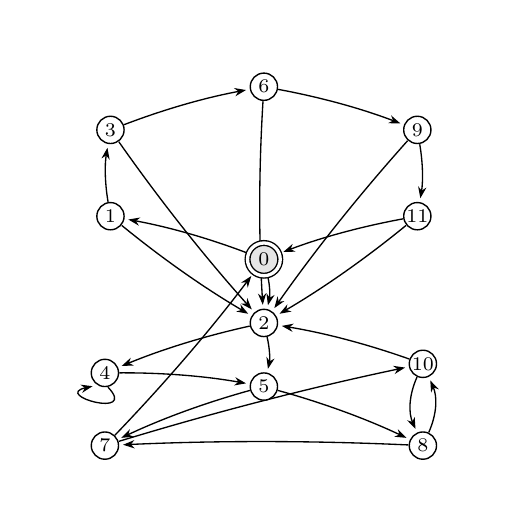
\begin{tikzpicture}[x=1cm,y=1cm,
  f1atlas state/.style={circle,draw=black,fill=white,line width=.5pt,inner sep=0pt,font=\fontsize{7}{8}\selectfont},
  f1atlas root/.style={f1atlas state,double,double distance=.42mm},
  f1atlas port0/.style={-{Stealth[length=1.45mm,width=1.05mm]},draw=black,line width=.48pt},
  f1atlas port1/.style={f1atlas port0},
  f1atlas label/.style={font=\fontsize{6}{7}\selectfont,fill=white,inner sep=.4pt}
]
\path[use as bounding box] (-3,-3) rectangle (3,3);
% edge 0 0 1
\draw[f1atlas port0] (-0.20478,0.13598) .. controls (-0.70112,0.32572) and (-1.20674,0.46830) .. (-1.72165,0.56372);
% edge 0 1 2
\draw[f1atlas port1] (0.04885,-0.15603) .. controls (0.07782,-0.28278) and (0.07868,-0.40578) .. (0.05142,-0.52503);
% edge 1 0 2
\draw[f1atlas port0] (-1.80565,0.48890) .. controls (-1.28655,0.06437) and (-0.75103,-0.30969) .. (-0.19908,-0.63328);
% edge 1 1 3
\draw[f1atlas port1] (-1.97922,0.78782) .. controls (-2.02032,1.03184) and (-2.02287,1.26068) .. (-1.98688,1.47436);
% edge 2 0 4
\draw[f1atlas port0] (-0.18027,-0.78984) .. controls (-0.75162,-0.91611) and (-1.29350,-1.08502) .. (-1.80592,-1.29656);
% edge 2 1 5
\draw[f1atlas port1] (0.04114,-0.92997) .. controls (0.07525,-1.07922) and (0.07868,-1.21347) .. (0.05142,-1.33272);
% edge 3 0 2
\draw[f1atlas port0] (-1.84240,1.55088) .. controls (-1.31183,0.79598) and (-0.74902,0.08632) .. (-0.15396,-0.57810);
% edge 3 1 6
\draw[f1atlas port1] (-1.77611,1.76785) .. controls (-1.25822,1.96583) and (-0.74182,2.11253) .. (-0.22691,2.20795);
% edge 4 0 4
\draw[f1atlas port0] (-1.98070,-1.56516) .. controls (-1.59080,-1.97187) and (-2.68847,-1.66841) .. (-2.17649,-1.55351);
% edge 4 1 5
\draw[f1atlas port1] (-1.83462,-1.38363) .. controls (-1.27936,-1.38067) and (-0.74355,-1.42519) .. (-0.22719,-1.51721);
% edge 5 0 7
\draw[f1atlas port0] (-0.17792,-1.60696) .. controls (-0.75381,-1.76643) and (-1.29802,-1.96716) .. (-1.81055,-2.20916);
% edge 5 1 8
\draw[f1atlas port1] (0.17792,-1.60696) .. controls (0.75381,-1.76643) and (1.29802,-1.96716) .. (1.81055,-2.20916);
% edge 6 0 2
\draw[f1atlas port0] (-0.01134,2.06573) .. controls (-0.06532,1.18858) and (-0.06626,0.32678) .. (-0.01417,-0.51967);
% edge 6 1 9
\draw[f1atlas port1] (0.18152,2.21636) .. controls (0.72669,2.11533) and (1.24385,1.97132) .. (1.73300,1.78433);
% edge 7 0 0
\draw[f1atlas port0] (-1.89126,-2.17463) .. controls (-1.25669,-1.51483) and (-0.67962,-0.84129) .. (-0.16004,-0.15401);
% edge 7 1 10
\draw[f1atlas port1] (-1.84264,-2.25385) .. controls (-0.62954,-1.88399) and (0.58248,-1.57163) .. (1.79341,-1.31676);
% edge 8 0 7
\draw[f1atlas port0] (1.83481,-2.29926) .. controls (0.61160,-2.24334) and (-0.59623,-2.24264) .. (-1.78870,-2.29715);
% edge 8 1 10
\draw[f1atlas port1] (2.09421,-2.13899) .. controls (2.19807,-1.90530) and (2.20432,-1.68568) .. (2.11296,-1.48011);
% edge 9 0 2
\draw[f1atlas port0] (1.82539,1.56440) .. controls (1.20980,0.87706) and (0.64557,0.16853) .. (0.13270,-0.56120);
% edge 9 1 11
\draw[f1atlas port1] (1.97922,1.51987) .. controls (2.02032,1.27585) and (2.02287,1.04701) .. (1.98688,0.83333);
% edge 10 0 2
\draw[f1atlas port0] (1.84518,-1.20766) .. controls (1.30346,-1.01603) and (0.76430,-0.87599) .. (0.22770,-0.78753);
% edge 10 1 8
\draw[f1atlas port1] (1.94425,-1.43793) .. controls (1.84039,-1.67162) and (1.83414,-1.89125) .. (1.92551,-2.09681);
% edge 11 0 0
\draw[f1atlas port0] (1.76703,0.57213) .. controls (1.22187,0.47110) and (0.71549,0.33121) .. (0.24789,0.15246);
% edge 11 1 2
\draw[f1atlas port1] (1.80565,0.48890) .. controls (1.28655,0.06437) and (0.75103,-0.30969) .. (0.19908,-0.63328);
% state 0
\node[f1atlas root,minimum size=4.1538mm,fill=black!10] (q0) at (0.00000,0.05769) {$ 0 $};
% state 1
\node[f1atlas state,minimum size=3.4615mm] (q1) at (-1.94856,0.60577) {$ 1 $};
% state 2
\node[f1atlas state,minimum size=3.4615mm] (q2) at (0.00000,-0.75000) {$ 2 $};
% state 3
\node[f1atlas state,minimum size=3.4615mm] (q3) at (-1.94856,1.70192) {$ 3 $};
% state 4
\node[f1atlas state,minimum size=3.4615mm] (q4) at (-2.01923,-1.38462) {$ 4 $};
% state 5
\node[f1atlas state,minimum size=3.4615mm] (q5) at (0.00000,-1.55769) {$ 5 $};
% state 6
\node[f1atlas state,minimum size=3.4615mm] (q6) at (-0.00000,2.25000) {$ 6 $};
% state 7
\node[f1atlas state,minimum size=3.4615mm] (q7) at (-2.01923,-2.30769) {$ 7 $};
% state 8
\node[f1atlas state,minimum size=3.4615mm] (q8) at (2.01923,-2.30769) {$ 8 $};
% state 9
\node[f1atlas state,minimum size=3.4615mm] (q9) at (1.94856,1.70192) {$ 9 $};
% state 10
\node[f1atlas state,minimum size=3.4615mm] (q10) at (2.01923,-1.26923) {$ 10 $};
% state 11
\node[f1atlas state,minimum size=3.4615mm] (q11) at (1.94856,0.60577) {$ 11 $};
\end{tikzpicture}
}\par
\small\textbf{(a)} Example start: $0$. Proved $H\ge34$.\\Exact score and global maximum unresolved.\par\end{minipage}
\clearpage
{\LARGE\bfseries $m=13$}\par\vspace{3mm}
\textbf{Constructive lower-bound example.} The indicated start gives $H\ge34$ by a static-mask projection onto a certified seven-state maximizer. This graph has not been certified globally optimal; its exact score is unresolved.\par\vspace{3mm}
\begin{minipage}[t]{.94\textwidth}\centering
\resizebox{10.3cm}{!}{% Family 1 rooted seed, m=13; key=0102020304050206040507080209001007100211020802120002.
% Requires \usepackage{tikz} and \usetikzlibrary{arrows.meta}.
% Score and global-maximality metadata belong in the surrounding caption.
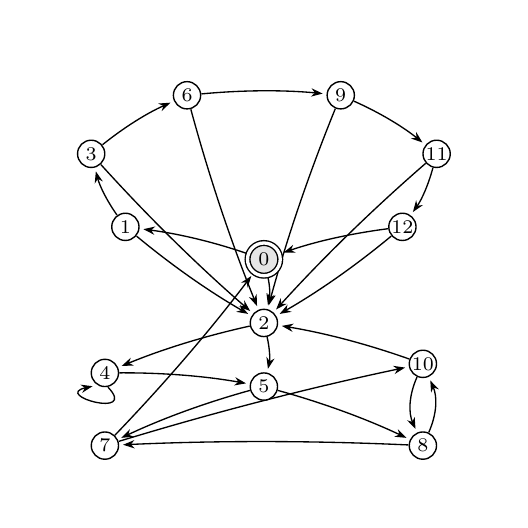
\begin{tikzpicture}[x=1cm,y=1cm,
  f1atlas state/.style={circle,draw=black,fill=white,line width=.5pt,inner sep=0pt,font=\fontsize{7}{8}\selectfont},
  f1atlas root/.style={f1atlas state,double,double distance=.42mm},
  f1atlas port0/.style={-{Stealth[length=1.45mm,width=1.05mm]},draw=black,line width=.48pt},
  f1atlas port1/.style={f1atlas port0},
  f1atlas label/.style={font=\fontsize{6}{7}\selectfont,fill=white,inner sep=.4pt}
]
\path[use as bounding box] (-3,-3) rectangle (3,3);
% edge 0 0 1
\draw[f1atlas port0] (-0.20724,0.12920) .. controls (-0.64140,0.27901) and (-1.08240,0.38288) .. (-1.53026,0.44080);
% edge 0 1 2
\draw[f1atlas port1] (0.04885,-0.15603) .. controls (0.07782,-0.28278) and (0.07868,-0.40578) .. (0.05142,-0.52503);
% edge 1 0 2
\draw[f1atlas port0] (-1.61704,0.35253) .. controls (-1.16046,-0.02625) and (-0.68819,-0.35550) .. (-0.20021,-0.63523);
% edge 1 1 3
\draw[f1atlas port1] (-1.86586,0.62104) .. controls (-1.99525,0.80363) and (-2.08473,0.98819) .. (-2.13431,1.17474);
% edge 2 0 4
\draw[f1atlas port0] (-0.18027,-0.78984) .. controls (-0.75162,-0.91611) and (-1.29350,-1.08502) .. (-1.80592,-1.29656);
% edge 2 1 5
\draw[f1atlas port1] (0.04114,-0.92997) .. controls (0.07525,-1.07922) and (0.07868,-1.21347) .. (0.05142,-1.33272);
% edge 3 0 2
\draw[f1atlas port0] (-2.06967,1.26092) .. controls (-1.46414,0.59226) and (-0.83234,-0.02763) .. (-0.17429,-0.59874);
% edge 3 1 6
\draw[f1atlas port1] (-2.04970,1.51343) .. controls (-1.77192,1.73673) and (-1.48435,1.91472) .. (-1.18698,2.04741);
% edge 4 0 4
\draw[f1atlas port0] (-1.98070,-1.56516) .. controls (-1.59080,-1.97187) and (-2.68847,-1.66841) .. (-2.17649,-1.55351);
% edge 4 1 5
\draw[f1atlas port1] (-1.83462,-1.38363) .. controls (-1.27936,-1.38067) and (-0.74355,-1.42519) .. (-0.22719,-1.51721);
% edge 5 0 7
\draw[f1atlas port0] (-0.17792,-1.60696) .. controls (-0.75381,-1.76643) and (-1.29802,-1.96716) .. (-1.81055,-2.20916);
% edge 5 1 8
\draw[f1atlas port1] (0.17792,-1.60696) .. controls (0.75381,-1.76643) and (1.29802,-1.96716) .. (1.81055,-2.20916);
% edge 6 0 2
\draw[f1atlas port0] (-0.92785,1.96329) .. controls (-0.69300,1.09856) and (-0.41268,0.26539) .. (-0.08689,-0.53621);
% edge 6 1 9
\draw[f1atlas port1] (-0.79244,2.15883) .. controls (-0.26415,2.20878) and (0.24883,2.21023) .. (0.74649,2.16317);
% edge 7 0 0
\draw[f1atlas port0] (-1.89126,-2.17463) .. controls (-1.25669,-1.51483) and (-0.67962,-0.84129) .. (-0.16004,-0.15401);
% edge 7 1 10
\draw[f1atlas port1] (-1.84264,-2.25385) .. controls (-0.62954,-1.88399) and (0.58248,-1.57163) .. (1.79341,-1.31676);
% edge 8 0 7
\draw[f1atlas port0] (1.83481,-2.29926) .. controls (0.61160,-2.24334) and (-0.59623,-2.24264) .. (-1.78870,-2.29715);
% edge 8 1 10
\draw[f1atlas port1] (2.09421,-2.13899) .. controls (2.19807,-1.90530) and (2.20432,-1.68568) .. (2.11296,-1.48011);
% edge 9 0 2
\draw[f1atlas port0] (0.90673,1.97042) .. controls (0.56935,1.14031) and (0.28727,0.30774) .. (0.06048,-0.52730);
% edge 9 1 11
\draw[f1atlas port1] (1.14483,2.06622) .. controls (1.47030,1.92099) and (1.75993,1.74637) .. (2.01373,1.54235);
% edge 10 0 2
\draw[f1atlas port0] (1.84518,-1.20766) .. controls (1.30346,-1.01603) and (0.76430,-0.87599) .. (0.22770,-0.78753);
% edge 10 1 8
\draw[f1atlas port1] (1.94425,-1.43793) .. controls (1.84039,-1.67162) and (1.83414,-1.89125) .. (1.92551,-2.09681);
% edge 11 0 2
\draw[f1atlas port0] (2.05416,1.27676) .. controls (1.37286,0.68548) and (0.73978,0.06691) .. (0.15490,-0.57895);
% edge 11 1 12
\draw[f1atlas port1] (2.14617,1.21934) .. controls (2.08868,1.00306) and (2.00414,0.81618) .. (1.89255,0.65869);
% edge 12 0 0
\draw[f1atlas port0] (1.57603,0.44672) .. controls (1.09766,0.38485) and (0.65594,0.28403) .. (0.25087,0.14426);
% edge 12 1 2
\draw[f1atlas port1] (1.61704,0.35253) .. controls (1.16046,-0.02625) and (0.68819,-0.35550) .. (0.20021,-0.63523);
% state 0
\node[f1atlas root,minimum size=4.1538mm,fill=black!10] (q0) at (0.00000,0.05769) {$ 0 $};
% state 1
\node[f1atlas state,minimum size=3.4615mm] (q1) at (-1.75912,0.47041) {$ 1 $};
% state 2
\node[f1atlas state,minimum size=3.4615mm] (q2) at (0.00000,-0.75000) {$ 2 $};
% state 3
\node[f1atlas state,minimum size=3.4615mm] (q3) at (-2.19359,1.39776) {$ 3 $};
% state 4
\node[f1atlas state,minimum size=3.4615mm] (q4) at (-2.01923,-1.38462) {$ 4 $};
% state 5
\node[f1atlas state,minimum size=3.4615mm] (q5) at (0.00000,-1.55769) {$ 5 $};
% state 6
\node[f1atlas state,minimum size=3.4615mm] (q6) at (-0.97624,2.14145) {$ 6 $};
% state 7
\node[f1atlas state,minimum size=3.4615mm] (q7) at (-2.01923,-2.30769) {$ 7 $};
% state 8
\node[f1atlas state,minimum size=3.4615mm] (q8) at (2.01923,-2.30769) {$ 8 $};
% state 9
\node[f1atlas state,minimum size=3.4615mm] (q9) at (0.97624,2.14145) {$ 9 $};
% state 10
\node[f1atlas state,minimum size=3.4615mm] (q10) at (2.01923,-1.26923) {$ 10 $};
% state 11
\node[f1atlas state,minimum size=3.4615mm] (q11) at (2.19359,1.39776) {$ 11 $};
% state 12
\node[f1atlas state,minimum size=3.4615mm] (q12) at (1.75912,0.47041) {$ 12 $};
\end{tikzpicture}
}\par
\small\textbf{(a)} Example start: $0$. Proved $H\ge34$.\\Exact score and global maximum unresolved.\par\end{minipage}
\clearpage
{\LARGE\bfseries $m=14$}\par\vspace{3mm}
\textbf{Constructive lower-bound example.} The indicated start gives $H\ge34$ by a static-mask projection onto a certified seven-state maximizer. This graph has not been certified globally optimal; its exact score is unresolved.\par\vspace{3mm}
\begin{minipage}[t]{.94\textwidth}\centering
\resizebox{10.3cm}{!}{% Family 1 rooted seed, m=14; key=01020203040502060405070802090010071002110208021202130002.
% Requires \usepackage{tikz} and \usetikzlibrary{arrows.meta}.
% Score and global-maximality metadata belong in the surrounding caption.
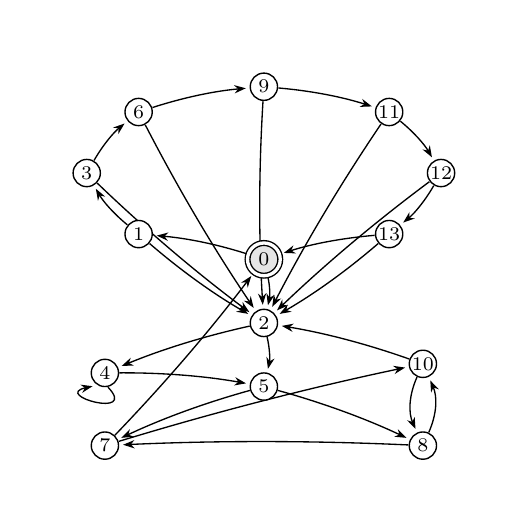
\begin{tikzpicture}[x=1cm,y=1cm,
  f1atlas state/.style={circle,draw=black,fill=white,line width=.5pt,inner sep=0pt,font=\fontsize{7}{8}\selectfont},
  f1atlas root/.style={f1atlas state,double,double distance=.42mm},
  f1atlas port0/.style={-{Stealth[length=1.45mm,width=1.05mm]},draw=black,line width=.48pt},
  f1atlas port1/.style={f1atlas port0},
  f1atlas label/.style={font=\fontsize{6}{7}\selectfont,fill=white,inner sep=.4pt}
]
\path[use as bounding box] (-3,-3) rectangle (3,3);
% edge 0 0 1
\draw[f1atlas port0] (-0.20862,0.12507) .. controls (-0.58770,0.24749) and (-0.97185,0.32546) .. (-1.36107,0.35896);
% edge 0 1 2
\draw[f1atlas port1] (0.04885,-0.15603) .. controls (0.07782,-0.28278) and (0.07868,-0.40578) .. (0.05142,-0.52503);
% edge 1 0 2
\draw[f1atlas port0] (-1.45115,0.25821) .. controls (-1.04966,-0.08787) and (-0.63259,-0.38554) .. (-0.19996,-0.63480);
% edge 1 1 3
\draw[f1atlas port1] (-1.73377,0.49579) .. controls (-1.90514,0.63627) and (-2.03865,0.78906) .. (-2.13431,0.95417);
% edge 2 0 4
\draw[f1atlas port0] (-0.18027,-0.78984) .. controls (-0.75162,-0.91611) and (-1.29350,-1.08502) .. (-1.80592,-1.29656);
% edge 2 1 5
\draw[f1atlas port1] (0.04114,-0.92997) .. controls (0.07525,-1.07922) and (0.07868,-1.21347) .. (0.05142,-1.33272);
% edge 3 0 2
\draw[f1atlas port0] (-2.11680,1.02602) .. controls (-1.49535,0.42964) and (-0.85146,-0.11644) .. (-0.18514,-0.61224);
% edge 3 1 6
\draw[f1atlas port1] (-2.15745,1.31359) .. controls (-2.04636,1.50532) and (-1.91703,1.66167) .. (-1.76946,1.78265);
% edge 4 0 4
\draw[f1atlas port0] (-1.98070,-1.56516) .. controls (-1.59080,-1.97187) and (-2.68847,-1.66841) .. (-2.17649,-1.55351);
% edge 4 1 5
\draw[f1atlas port1] (-1.83462,-1.38363) .. controls (-1.27936,-1.38067) and (-0.74355,-1.42519) .. (-0.22719,-1.51721);
% edge 5 0 7
\draw[f1atlas port0] (-0.17792,-1.60696) .. controls (-0.75381,-1.76643) and (-1.29802,-1.96716) .. (-1.81055,-2.20916);
% edge 5 1 8
\draw[f1atlas port1] (0.17792,-1.60696) .. controls (0.75381,-1.76643) and (1.29802,-1.96716) .. (1.81055,-2.20916);
% edge 6 0 2
\draw[f1atlas port0] (-1.50627,1.76491) .. controls (-1.08533,0.94986) and (-0.62636,0.17526) .. (-0.12937,-0.55890);
% edge 6 1 9
\draw[f1atlas port1] (-1.41531,1.98568) .. controls (-1.01427,2.11520) and (-0.61914,2.19671) .. (-0.22992,2.23021);
% edge 7 0 0
\draw[f1atlas port0] (-1.89126,-2.17463) .. controls (-1.25669,-1.51483) and (-0.67962,-0.84129) .. (-0.16004,-0.15401);
% edge 7 1 10
\draw[f1atlas port1] (-1.84264,-2.25385) .. controls (-0.62954,-1.88399) and (0.58248,-1.57163) .. (1.79341,-1.31676);
% edge 8 0 7
\draw[f1atlas port0] (1.83481,-2.29926) .. controls (0.61160,-2.24334) and (-0.59623,-2.24264) .. (-1.78870,-2.29715);
% edge 8 1 10
\draw[f1atlas port1] (2.09421,-2.13899) .. controls (2.19807,-1.90530) and (2.20432,-1.68568) .. (2.11296,-1.48011);
% edge 9 0 2
\draw[f1atlas port0] (-0.01134,2.06573) .. controls (-0.06532,1.18858) and (-0.06626,0.32678) .. (-0.01417,-0.51967);
% edge 9 1 11
\draw[f1atlas port1] (0.18394,2.23417) .. controls (0.60381,2.19803) and (0.99963,2.11993) .. (1.37139,1.99987);
% edge 10 0 2
\draw[f1atlas port0] (1.84518,-1.20766) .. controls (1.30346,-1.01603) and (0.76430,-0.87599) .. (0.22770,-0.78753);
% edge 10 1 8
\draw[f1atlas port1] (1.94425,-1.43793) .. controls (1.84039,-1.67162) and (1.83414,-1.89125) .. (1.92551,-2.09681);
% edge 11 0 2
\draw[f1atlas port0] (1.48750,1.77606) .. controls (0.97325,1.01643) and (0.51272,0.24275) .. (0.10589,-0.54496);
% edge 11 1 12
\draw[f1atlas port1] (1.73377,1.81191) .. controls (1.90514,1.67143) and (2.03865,1.51863) .. (2.13431,1.35352);
% edge 12 0 2
\draw[f1atlas port0] (2.10189,1.04364) .. controls (1.41088,0.52947) and (0.76575,-0.01515) .. (0.16650,-0.59022);
% edge 12 1 13
\draw[f1atlas port1] (2.15745,0.99411) .. controls (2.04636,0.80237) and (1.91703,0.64602) .. (1.76946,0.52505);
% edge 13 0 0
\draw[f1atlas port0] (1.40706,0.36292) .. controls (0.98718,0.32677) and (0.60234,0.25222) .. (0.25254,0.13925);
% edge 13 1 2
\draw[f1atlas port1] (1.45115,0.25821) .. controls (1.04966,-0.08787) and (0.63259,-0.38554) .. (0.19996,-0.63480);
% state 0
\node[f1atlas root,minimum size=4.1538mm,fill=black!10] (q0) at (0.00000,0.05769) {$ 0 $};
% state 1
\node[f1atlas state,minimum size=3.4615mm] (q1) at (-1.59099,0.37875) {$ 1 $};
% state 2
\node[f1atlas state,minimum size=3.4615mm] (q2) at (0.00000,-0.75000) {$ 2 $};
% state 3
\node[f1atlas state,minimum size=3.4615mm] (q3) at (-2.25000,1.15385) {$ 3 $};
% state 4
\node[f1atlas state,minimum size=3.4615mm] (q4) at (-2.01923,-1.38462) {$ 4 $};
% state 5
\node[f1atlas state,minimum size=3.4615mm] (q5) at (0.00000,-1.55769) {$ 5 $};
% state 6
\node[f1atlas state,minimum size=3.4615mm] (q6) at (-1.59099,1.92894) {$ 6 $};
% state 7
\node[f1atlas state,minimum size=3.4615mm] (q7) at (-2.01923,-2.30769) {$ 7 $};
% state 8
\node[f1atlas state,minimum size=3.4615mm] (q8) at (2.01923,-2.30769) {$ 8 $};
% state 9
\node[f1atlas state,minimum size=3.4615mm] (q9) at (-0.00000,2.25000) {$ 9 $};
% state 10
\node[f1atlas state,minimum size=3.4615mm] (q10) at (2.01923,-1.26923) {$ 10 $};
% state 11
\node[f1atlas state,minimum size=3.4615mm] (q11) at (1.59099,1.92894) {$ 11 $};
% state 12
\node[f1atlas state,minimum size=3.4615mm] (q12) at (2.25000,1.15385) {$ 12 $};
% state 13
\node[f1atlas state,minimum size=3.4615mm] (q13) at (1.59099,0.37875) {$ 13 $};
\end{tikzpicture}
}\par
\small\textbf{(a)} Example start: $0$. Proved $H\ge34$.\\Exact score and global maximum unresolved.\par\end{minipage}
\clearpage
{\LARGE\bfseries $m=15$}\par\vspace{3mm}
\textbf{Constructive lower-bound example.} The indicated start gives $H\ge34$ by a static-mask projection onto a certified seven-state maximizer. This graph has not been certified globally optimal; its exact score is unresolved.\par\vspace{3mm}
\begin{minipage}[t]{.94\textwidth}\centering
\resizebox{10.3cm}{!}{% Family 1 rooted seed, m=15; key=010202030405020604050708020900100710021102080212021302140002.
% Requires \usepackage{tikz} and \usetikzlibrary{arrows.meta}.
% Score and global-maximality metadata belong in the surrounding caption.
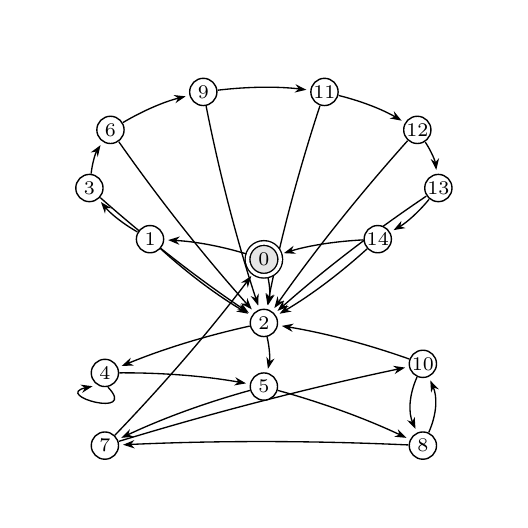
\begin{tikzpicture}[x=1cm,y=1cm,
  f1atlas state/.style={circle,draw=black,fill=white,line width=.5pt,inner sep=0pt,font=\fontsize{7}{8}\selectfont},
  f1atlas root/.style={f1atlas state,double,double distance=.42mm},
  f1atlas port0/.style={-{Stealth[length=1.45mm,width=1.05mm]},draw=black,line width=.48pt},
  f1atlas port1/.style={f1atlas port0},
  f1atlas label/.style={font=\fontsize{6}{7}\selectfont,fill=white,inner sep=.4pt}
]
\path[use as bounding box] (-3,-3) rectangle (3,3);
% edge 0 0 1
\draw[f1atlas port0] (-0.20940,0.12259) .. controls (-0.54115,0.22540) and (-0.87661,0.28537) .. (-1.21580,0.30250);
% edge 0 1 2
\draw[f1atlas port1] (0.04885,-0.15603) .. controls (0.07782,-0.28278) and (0.07868,-0.40578) .. (0.05142,-0.52503);
% edge 1 0 2
\draw[f1atlas port0] (-1.30954,0.19010) .. controls (-0.95508,-0.13149) and (-0.58486,-0.40584) .. (-0.19889,-0.63296);
% edge 1 1 3
\draw[f1atlas port1] (-1.60653,0.40580) .. controls (-1.79589,0.51412) and (-1.95011,0.64062) .. (-2.06918,0.78531);
% edge 2 0 4
\draw[f1atlas port0] (-0.18027,-0.78984) .. controls (-0.75162,-0.91611) and (-1.29350,-1.08502) .. (-1.80592,-1.29656);
% edge 2 1 5
\draw[f1atlas port1] (0.04114,-0.92997) .. controls (0.07525,-1.07922) and (0.07868,-1.21347) .. (0.05142,-1.33272);
% edge 3 0 2
\draw[f1atlas port0] (-2.07752,0.84121) .. controls (-1.46876,0.30289) and (-0.84007,-0.18456) .. (-0.19144,-0.62114);
% edge 3 1 6
\draw[f1atlas port1] (-2.19438,1.14687) .. controls (-2.17745,1.29171) and (-2.13755,1.41231) .. (-2.07467,1.50866);
% edge 4 0 4
\draw[f1atlas port0] (-1.98070,-1.56516) .. controls (-1.59080,-1.97187) and (-2.68847,-1.66841) .. (-2.17649,-1.55351);
% edge 4 1 5
\draw[f1atlas port1] (-1.83462,-1.38363) .. controls (-1.27936,-1.38067) and (-0.74355,-1.42519) .. (-0.22719,-1.51721);
% edge 5 0 7
\draw[f1atlas port0] (-0.17792,-1.60696) .. controls (-0.75381,-1.76643) and (-1.29802,-1.96716) .. (-1.81055,-2.20916);
% edge 5 1 8
\draw[f1atlas port1] (0.17792,-1.60696) .. controls (0.75381,-1.76643) and (1.29802,-1.96716) .. (1.81055,-2.20916);
% edge 6 0 2
\draw[f1atlas port0] (-1.84240,1.55088) .. controls (-1.31183,0.79598) and (-0.74902,0.08632) .. (-0.15396,-0.57810);
% edge 6 1 9
\draw[f1atlas port1] (-1.78946,1.79557) .. controls (-1.52581,1.95076) and (-1.26048,2.06161) .. (-0.99347,2.12812);
% edge 7 0 0
\draw[f1atlas port0] (-1.89126,-2.17463) .. controls (-1.25669,-1.51483) and (-0.67962,-0.84129) .. (-0.16004,-0.15401);
% edge 7 1 10
\draw[f1atlas port1] (-1.84264,-2.25385) .. controls (-0.62954,-1.88399) and (0.58248,-1.57163) .. (1.79341,-1.31676);
% edge 8 0 7
\draw[f1atlas port0] (1.83481,-2.29926) .. controls (0.61160,-2.24334) and (-0.59623,-2.24264) .. (-1.78870,-2.29715);
% edge 8 1 10
\draw[f1atlas port1] (2.09421,-2.13899) .. controls (2.19807,-1.90530) and (2.20432,-1.68568) .. (2.11296,-1.48011);
% edge 9 0 2
\draw[f1atlas port0] (-0.73364,2.00280) .. controls (-0.56059,1.12995) and (-0.34004,0.28543) .. (-0.07200,-0.53075);
% edge 9 1 11
\draw[f1atlas port1] (-0.58624,2.20588) .. controls (-0.19541,2.25276) and (0.18014,2.25459) .. (0.54042,2.21138);
% edge 10 0 2
\draw[f1atlas port0] (1.84518,-1.20766) .. controls (1.30346,-1.01603) and (0.76430,-0.87599) .. (0.22770,-0.78753);
% edge 10 1 8
\draw[f1atlas port1] (1.94425,-1.43793) .. controls (1.84039,-1.67162) and (1.83414,-1.89125) .. (1.92551,-2.09681);
% edge 11 0 2
\draw[f1atlas port0] (0.71194,2.00849) .. controls (0.43430,1.16308) and (0.21195,0.31903) .. (0.04488,-0.52364);
% edge 11 1 12
\draw[f1atlas port1] (0.94869,2.13927) .. controls (1.24555,2.06533) and (1.51255,1.95856) .. (1.74968,1.81898);
% edge 12 0 2
\draw[f1atlas port0] (1.82539,1.56440) .. controls (1.20980,0.87706) and (0.64557,0.16853) .. (0.13270,-0.56120);
% edge 12 1 13
\draw[f1atlas port1] (2.04945,1.54731) .. controls (2.12914,1.42519) and (2.17566,1.30699) .. (2.18902,1.19271);
% edge 13 0 2
\draw[f1atlas port0] (2.06266,0.86041) .. controls (1.38852,0.40665) and (0.75859,-0.07920) .. (0.17287,-0.59713);
% edge 13 1 14
\draw[f1atlas port1] (2.09851,0.82095) .. controls (1.95989,0.65250) and (1.80925,0.52176) .. (1.64659,0.42872);
% edge 14 0 0
\draw[f1atlas port0] (1.26189,0.30483) .. controls (0.89198,0.28615) and (0.55584,0.22996) .. (0.25349,0.13625);
% edge 14 1 2
\draw[f1atlas port1] (1.30954,0.19010) .. controls (0.95508,-0.13149) and (0.58486,-0.40584) .. (0.19889,-0.63296);
% state 0
\node[f1atlas root,minimum size=4.1538mm,fill=black!10] (q0) at (0.00000,0.05769) {$ 0 $};
% state 1
\node[f1atlas state,minimum size=3.4615mm] (q1) at (-1.44627,0.31414) {$ 1 $};
% state 2
\node[f1atlas state,minimum size=3.4615mm] (q2) at (0.00000,-0.75000) {$ 2 $};
% state 3
\node[f1atlas state,minimum size=3.4615mm] (q3) at (-2.21582,0.96350) {$ 3 $};
% state 4
\node[f1atlas state,minimum size=3.4615mm] (q4) at (-2.01923,-1.38462) {$ 4 $};
% state 5
\node[f1atlas state,minimum size=3.4615mm] (q5) at (0.00000,-1.55769) {$ 5 $};
% state 6
\node[f1atlas state,minimum size=3.4615mm] (q6) at (-1.94856,1.70192) {$ 6 $};
% state 7
\node[f1atlas state,minimum size=3.4615mm] (q7) at (-2.01923,-2.30769) {$ 7 $};
% state 8
\node[f1atlas state,minimum size=3.4615mm] (q8) at (2.01923,-2.30769) {$ 8 $};
% state 9
\node[f1atlas state,minimum size=3.4615mm] (q9) at (-0.76955,2.18389) {$ 9 $};
% state 10
\node[f1atlas state,minimum size=3.4615mm] (q10) at (2.01923,-1.26923) {$ 10 $};
% state 11
\node[f1atlas state,minimum size=3.4615mm] (q11) at (0.76955,2.18389) {$ 11 $};
% state 12
\node[f1atlas state,minimum size=3.4615mm] (q12) at (1.94856,1.70192) {$ 12 $};
% state 13
\node[f1atlas state,minimum size=3.4615mm] (q13) at (2.21582,0.96350) {$ 13 $};
% state 14
\node[f1atlas state,minimum size=3.4615mm] (q14) at (1.44627,0.31414) {$ 14 $};
\end{tikzpicture}
}\par
\small\textbf{(a)} Example start: $0$. Proved $H\ge34$.\\Exact score and global maximum unresolved.\par\end{minipage}
\clearpage
{\LARGE\bfseries $m=16$}\par\vspace{3mm}
\textbf{Constructive lower-bound example.} The indicated start gives $H\ge34$ by a static-mask projection onto a certified seven-state maximizer. This graph has not been certified globally optimal; its exact score is unresolved.\par\vspace{3mm}
\begin{minipage}[t]{.94\textwidth}\centering
\resizebox{10.3cm}{!}{% Family 1 rooted seed, m=16; key=0102020304050206040507080209001007100211020802120213021402150002.
% Requires \usepackage{tikz} and \usetikzlibrary{arrows.meta}.
% Score and global-maximality metadata belong in the surrounding caption.
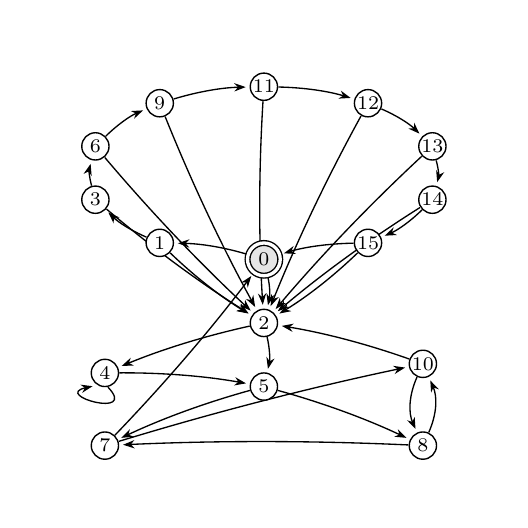
\begin{tikzpicture}[x=1cm,y=1cm,
  f1atlas state/.style={circle,draw=black,fill=white,line width=.5pt,inner sep=0pt,font=\fontsize{7}{8}\selectfont},
  f1atlas root/.style={f1atlas state,double,double distance=.42mm},
  f1atlas port0/.style={-{Stealth[length=1.45mm,width=1.05mm]},draw=black,line width=.48pt},
  f1atlas port1/.style={f1atlas port0},
  f1atlas label/.style={font=\fontsize{6}{7}\selectfont,fill=white,inner sep=.4pt}
]
\path[use as bounding box] (-3,-3) rectangle (3,3);
% edge 0 0 1
\draw[f1atlas port0] (-0.20982,0.12122) .. controls (-0.50116,0.20943) and (-0.79515,0.25650) .. (-1.09179,0.26243);
% edge 0 1 2
\draw[f1atlas port1] (0.04885,-0.15603) .. controls (0.07782,-0.28278) and (0.07868,-0.40578) .. (0.05142,-0.52503);
% edge 1 0 2
\draw[f1atlas port0] (-1.18944,0.13908) .. controls (-0.87483,-0.16341) and (-0.54412,-0.41987) .. (-0.19729,-0.63030);
% edge 1 1 3
\draw[f1atlas port1] (-1.49218,0.33982) .. controls (-1.68580,0.42288) and (-1.84680,0.52743) .. (-1.97519,0.65346);
% edge 2 0 4
\draw[f1atlas port0] (-0.18027,-0.78984) .. controls (-0.75162,-0.91611) and (-1.29350,-1.08502) .. (-1.80592,-1.29656);
% edge 2 1 5
\draw[f1atlas port1] (0.04114,-0.92997) .. controls (0.07525,-1.07922) and (0.07868,-1.21347) .. (0.05142,-1.33272);
% edge 3 0 2
\draw[f1atlas port0] (-1.99880,0.69604) .. controls (-1.41589,0.20405) and (-0.81471,-0.23698) .. (-0.19528,-0.62703);
% edge 3 1 6
\draw[f1atlas port1] (-2.18842,0.99324) .. controls (-2.21760,1.10031) and (-2.22164,1.19254) .. (-2.20055,1.26993);
% edge 4 0 4
\draw[f1atlas port0] (-1.98070,-1.56516) .. controls (-1.59080,-1.97187) and (-2.68847,-1.66841) .. (-2.17649,-1.55351);
% edge 4 1 5
\draw[f1atlas port1] (-1.83462,-1.38363) .. controls (-1.27936,-1.38067) and (-0.74355,-1.42519) .. (-0.22719,-1.51721);
% edge 5 0 7
\draw[f1atlas port0] (-0.17792,-1.60696) .. controls (-0.75381,-1.76643) and (-1.29802,-1.96716) .. (-1.81055,-2.20916);
% edge 5 1 8
\draw[f1atlas port1] (0.17792,-1.60696) .. controls (0.75381,-1.76643) and (1.29802,-1.96716) .. (1.81055,-2.20916);
% edge 6 0 2
\draw[f1atlas port0] (-2.02059,1.35167) .. controls (-1.43135,0.65560) and (-0.81413,0.00744) .. (-0.16896,-0.59281);
% edge 6 1 9
\draw[f1atlas port1] (-2.00813,1.62190) .. controls (-1.85778,1.76949) and (-1.69994,1.87875) .. (-1.53460,1.94967);
% edge 7 0 0
\draw[f1atlas port0] (-1.89126,-2.17463) .. controls (-1.25669,-1.51483) and (-0.67962,-0.84129) .. (-0.16004,-0.15401);
% edge 7 1 10
\draw[f1atlas port1] (-1.84264,-2.25385) .. controls (-0.62954,-1.88399) and (0.58248,-1.57163) .. (1.79341,-1.31676);
% edge 8 0 7
\draw[f1atlas port0] (1.83481,-2.29926) .. controls (0.61160,-2.24334) and (-0.59623,-2.24264) .. (-1.78870,-2.29715);
% edge 8 1 10
\draw[f1atlas port1] (2.09421,-2.13899) .. controls (2.19807,-1.90530) and (2.20432,-1.68568) .. (2.11296,-1.48011);
% edge 9 0 2
\draw[f1atlas port0] (-1.25355,1.86940) .. controls (-0.91430,1.02700) and (-0.53348,0.22129) .. (-0.11110,-0.54773);
% edge 9 1 11
\draw[f1atlas port1] (-1.14582,2.09415) .. controls (-0.83240,2.18905) and (-0.52737,2.23946) .. (-0.23072,2.24539);
% edge 10 0 2
\draw[f1atlas port0] (1.84518,-1.20766) .. controls (1.30346,-1.01603) and (0.76430,-0.87599) .. (0.22770,-0.78753);
% edge 10 1 8
\draw[f1atlas port1] (1.94425,-1.43793) .. controls (1.84039,-1.67162) and (1.83414,-1.89125) .. (1.92551,-2.09681);
% edge 11 0 2
\draw[f1atlas port0] (-0.01134,2.06573) .. controls (-0.06532,1.18858) and (-0.06626,0.32678) .. (-0.01417,-0.51967);
% edge 11 1 12
\draw[f1atlas port1] (0.18458,2.24631) .. controls (0.51199,2.23977) and (0.81768,2.19351) .. (1.10165,2.10753);
% edge 12 0 2
\draw[f1atlas port0] (1.23364,1.87884) .. controls (0.79644,1.08285) and (0.41396,0.27793) .. (0.08621,-0.53594);
% edge 12 1 13
\draw[f1atlas port1] (1.49218,1.96787) .. controls (1.68580,1.88481) and (1.84680,1.78027) .. (1.97519,1.65423);
% edge 13 0 2
\draw[f1atlas port0] (2.00471,1.36682) .. controls (1.33701,0.74562) and (0.71847,0.09872) .. (0.14910,-0.57387);
% edge 13 1 14
\draw[f1atlas port1] (2.18842,1.31446) .. controls (2.21760,1.20738) and (2.22164,1.11515) .. (2.20055,1.03777);
% edge 14 0 2
\draw[f1atlas port0] (1.98365,0.71674) .. controls (1.33818,0.31029) and (0.73575,-0.12901) .. (0.17635,-0.60115);
% edge 14 1 15
\draw[f1atlas port1] (2.00813,0.68579) .. controls (1.85778,0.53820) and (1.69994,0.42895) .. (1.53460,0.35802);
% edge 15 0 0
\draw[f1atlas port0] (1.13794,0.26335) .. controls (0.81053,0.25681) and (0.51588,0.21389) .. (0.25400,0.13460);
% edge 15 1 2
\draw[f1atlas port1] (1.18944,0.13908) .. controls (0.87483,-0.16341) and (0.54412,-0.41987) .. (0.19729,-0.63030);
% state 0
\node[f1atlas root,minimum size=4.1538mm,fill=black!10] (q0) at (0.00000,0.05769) {$ 0 $};
% state 1
\node[f1atlas state,minimum size=3.4615mm] (q1) at (-1.32252,0.26704) {$ 1 $};
% state 2
\node[f1atlas state,minimum size=3.4615mm] (q2) at (0.00000,-0.75000) {$ 2 $};
% state 3
\node[f1atlas state,minimum size=3.4615mm] (q3) at (-2.13988,0.81512) {$ 3 $};
% state 4
\node[f1atlas state,minimum size=3.4615mm] (q4) at (-2.01923,-1.38462) {$ 4 $};
% state 5
\node[f1atlas state,minimum size=3.4615mm] (q5) at (0.00000,-1.55769) {$ 5 $};
% state 6
\node[f1atlas state,minimum size=3.4615mm] (q6) at (-2.13988,1.49258) {$ 6 $};
% state 7
\node[f1atlas state,minimum size=3.4615mm] (q7) at (-2.01923,-2.30769) {$ 7 $};
% state 8
\node[f1atlas state,minimum size=3.4615mm] (q8) at (2.01923,-2.30769) {$ 8 $};
% state 9
\node[f1atlas state,minimum size=3.4615mm] (q9) at (-1.32252,2.04065) {$ 9 $};
% state 10
\node[f1atlas state,minimum size=3.4615mm] (q10) at (2.01923,-1.26923) {$ 10 $};
% state 11
\node[f1atlas state,minimum size=3.4615mm] (q11) at (-0.00000,2.25000) {$ 11 $};
% state 12
\node[f1atlas state,minimum size=3.4615mm] (q12) at (1.32252,2.04065) {$ 12 $};
% state 13
\node[f1atlas state,minimum size=3.4615mm] (q13) at (2.13988,1.49258) {$ 13 $};
% state 14
\node[f1atlas state,minimum size=3.4615mm] (q14) at (2.13988,0.81512) {$ 14 $};
% state 15
\node[f1atlas state,minimum size=3.4615mm] (q15) at (1.32252,0.26704) {$ 15 $};
\end{tikzpicture}
}\par
\small\textbf{(a)} Example start: $0$. Proved $H\ge34$.\\Exact score and global maximum unresolved.\par\end{minipage}
\clearpage
{\LARGE\bfseries $m=17$}\par\vspace{3mm}
\textbf{Constructive lower-bound example.} The indicated start gives $H\ge34$ by a static-mask projection onto a certified seven-state maximizer. This graph has not been certified globally optimal; its exact score is unresolved.\par\vspace{3mm}
\begin{minipage}[t]{.94\textwidth}\centering
\resizebox{10.3cm}{!}{% Family 1 rooted seed, m=17; key=01020203040502060405070802090010071002110208021202130214021502160002.
% Requires \usepackage{tikz} and \usetikzlibrary{arrows.meta}.
% Score and global-maximality metadata belong in the surrounding caption.
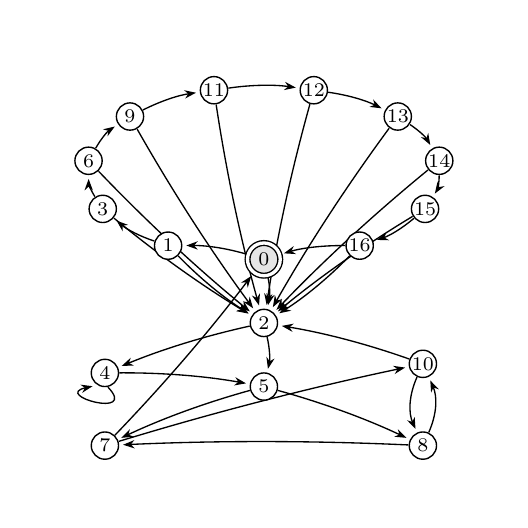
\begin{tikzpicture}[x=1cm,y=1cm,
  f1atlas state/.style={circle,draw=black,fill=white,line width=.5pt,inner sep=0pt,font=\fontsize{7}{8}\selectfont},
  f1atlas root/.style={f1atlas state,double,double distance=.42mm},
  f1atlas port0/.style={-{Stealth[length=1.45mm,width=1.05mm]},draw=black,line width=.48pt},
  f1atlas port1/.style={f1atlas port0},
  f1atlas label/.style={font=\fontsize{6}{7}\selectfont,fill=white,inner sep=.4pt}
]
\path[use as bounding box] (-3,-3) rectangle (3,3);
% edge 0 0 1
\draw[f1atlas port0] (-0.21000,0.12064) .. controls (-0.46677,0.19760) and (-0.72533,0.23516) .. (-0.98568,0.23333);
% edge 0 1 2
\draw[f1atlas port1] (0.04885,-0.15603) .. controls (0.07782,-0.28278) and (0.07868,-0.40578) .. (0.05142,-0.52503);
% edge 1 0 2
\draw[f1atlas port0] (-1.08737,0.09971) .. controls (-0.80658,-0.18742) and (-0.50924,-0.42970) .. (-0.19534,-0.62713);
% edge 1 1 3
\draw[f1atlas port1] (-1.39164,0.28990) .. controls (-1.58174,0.35306) and (-1.74143,0.43948) .. (-1.87071,0.54918);
% edge 2 0 4
\draw[f1atlas port0] (-0.18027,-0.78984) .. controls (-0.75162,-0.91611) and (-1.29350,-1.08502) .. (-1.80592,-1.29656);
% edge 2 1 5
\draw[f1atlas port1] (0.04114,-0.92997) .. controls (0.07525,-1.07922) and (0.07868,-1.21347) .. (0.05142,-1.33272);
% edge 3 0 2
\draw[f1atlas port0] (-1.90422,0.58106) .. controls (-1.35251,0.12628) and (-0.78366,-0.27770) .. (-0.19765,-0.63088);
% edge 3 1 6
\draw[f1atlas port1] (-2.14612,0.85403) .. controls (-2.19899,0.93670) and (-2.22559,1.01172) .. (-2.22593,1.07908);
% edge 4 0 4
\draw[f1atlas port0] (-1.98070,-1.56516) .. controls (-1.59080,-1.97187) and (-2.68847,-1.66841) .. (-2.17649,-1.55351);
% edge 4 1 5
\draw[f1atlas port1] (-1.83462,-1.38363) .. controls (-1.27936,-1.38067) and (-0.74355,-1.42519) .. (-0.22719,-1.51721);
% edge 5 0 7
\draw[f1atlas port0] (-0.17792,-1.60696) .. controls (-0.75381,-1.76643) and (-1.29802,-1.96716) .. (-1.81055,-2.20916);
% edge 5 1 8
\draw[f1atlas port1] (0.17792,-1.60696) .. controls (0.75381,-1.76643) and (1.29802,-1.96716) .. (1.81055,-2.20916);
% edge 6 0 2
\draw[f1atlas port0] (-2.09943,1.17649) .. controls (-1.48396,0.53360) and (-0.84369,-0.05986) .. (-0.17862,-0.60389);
% edge 6 1 9
\draw[f1atlas port1] (-2.13572,1.47026) .. controls (-2.06598,1.59268) and (-1.98513,1.68417) .. (-1.89316,1.74474);
% edge 7 0 0
\draw[f1atlas port0] (-1.89126,-2.17463) .. controls (-1.25669,-1.51483) and (-0.67962,-0.84129) .. (-0.16004,-0.15401);
% edge 7 1 10
\draw[f1atlas port1] (-1.84264,-2.25385) .. controls (-0.62954,-1.88399) and (0.58248,-1.57163) .. (1.79341,-1.31676);
% edge 8 0 7
\draw[f1atlas port0] (1.83481,-2.29926) .. controls (0.61160,-2.24334) and (-0.59623,-2.24264) .. (-1.78870,-2.29715);
% edge 8 1 10
\draw[f1atlas port1] (2.09421,-2.13899) .. controls (2.19807,-1.90530) and (2.20432,-1.68568) .. (2.11296,-1.48011);
% edge 9 0 2
\draw[f1atlas port0] (-1.60928,1.71113) .. controls (-1.15487,0.91078) and (-0.66403,0.15236) .. (-0.13678,-0.56413);
% edge 9 1 11
\draw[f1atlas port1] (-1.53560,1.95481) .. controls (-1.30837,2.06942) and (-1.08397,2.14231) .. (-0.86242,2.17346);
% edge 10 0 2
\draw[f1atlas port0] (1.84518,-1.20766) .. controls (1.30346,-1.01603) and (0.76430,-0.87599) .. (0.22770,-0.78753);
% edge 10 1 8
\draw[f1atlas port1] (1.94425,-1.43793) .. controls (1.84039,-1.67162) and (1.83414,-1.89125) .. (1.92551,-2.09681);
% edge 11 0 2
\draw[f1atlas port0] (-0.60626,2.02306) .. controls (-0.47356,1.14665) and (-0.29216,0.29638) .. (-0.06206,-0.52773);
% edge 11 1 12
\draw[f1atlas port1] (-0.45121,2.23220) .. controls (-0.15040,2.27600) and (0.13518,2.27822) .. (0.40554,2.23885);
% edge 12 0 2
\draw[f1atlas port0] (0.58425,2.02778) .. controls (0.34588,1.17403) and (0.16265,0.32416) .. (0.03455,-0.52183);
% edge 12 1 13
\draw[f1atlas port1] (0.81671,2.17989) .. controls (1.06874,2.14445) and (1.29463,2.07635) .. (1.49439,1.97560);
% edge 13 0 2
\draw[f1atlas port0] (1.59102,1.72298) .. controls (1.04552,0.98171) and (0.55316,0.22427) .. (0.11394,-0.54932);
% edge 13 1 14
\draw[f1atlas port1] (1.85462,1.77013) .. controls (1.97228,1.69264) and (2.05837,1.60605) .. (2.11287,1.51036);
% edge 14 0 2
\draw[f1atlas port0] (2.08420,1.19296) .. controls (1.39532,0.62944) and (0.75378,0.03736) .. (0.15958,-0.58331);
% edge 14 1 15
\draw[f1atlas port1] (2.22616,1.12523) .. controls (2.22567,1.02710) and (2.20727,0.94966) .. (2.17099,0.89291);
% edge 15 0 2
\draw[f1atlas port0] (1.88855,0.60319) .. controls (1.27619,0.23412) and (0.70603,-0.16801) .. (0.17807,-0.60322);
% edge 15 1 16
\draw[f1atlas port1] (1.90590,0.57904) .. controls (1.75317,0.44944) and (1.59634,0.35791) .. (1.43544,0.30446);
% edge 16 0 0
\draw[f1atlas port0] (1.03183,0.23300) .. controls (0.74071,0.23505) and (0.48150,0.20201) .. (0.25421,0.13389);
% edge 16 1 2
\draw[f1atlas port1] (1.08737,0.09971) .. controls (0.80658,-0.18742) and (0.50924,-0.42970) .. (0.19534,-0.62713);
% state 0
\node[f1atlas root,minimum size=4.1538mm,fill=black!10] (q0) at (0.00000,0.05769) {$ 0 $};
% state 1
\node[f1atlas state,minimum size=3.4615mm] (q1) at (-1.21644,0.23170) {$ 1 $};
% state 2
\node[f1atlas state,minimum size=3.4615mm] (q2) at (0.00000,-0.75000) {$ 2 $};
% state 3
\node[f1atlas state,minimum size=3.4615mm] (q3) at (-2.04667,0.69849) {$ 3 $};
% state 4
\node[f1atlas state,minimum size=3.4615mm] (q4) at (-2.01923,-1.38462) {$ 4 $};
% state 5
\node[f1atlas state,minimum size=3.4615mm] (q5) at (0.00000,-1.55769) {$ 5 $};
% state 6
\node[f1atlas state,minimum size=3.4615mm] (q6) at (-2.22710,1.30985) {$ 6 $};
% state 7
\node[f1atlas state,minimum size=3.4615mm] (q7) at (-2.01923,-2.30769) {$ 7 $};
% state 8
\node[f1atlas state,minimum size=3.4615mm] (q8) at (2.01923,-2.30769) {$ 8 $};
% state 9
\node[f1atlas state,minimum size=3.4615mm] (q9) at (-1.70044,1.87167) {$ 9 $};
% state 10
\node[f1atlas state,minimum size=3.4615mm] (q10) at (2.01923,-1.26923) {$ 10 $};
% state 11
\node[f1atlas state,minimum size=3.4615mm] (q11) at (-0.63390,2.20560) {$ 11 $};
% state 12
\node[f1atlas state,minimum size=3.4615mm] (q12) at (0.63390,2.20560) {$ 12 $};
% state 13
\node[f1atlas state,minimum size=3.4615mm] (q13) at (1.70044,1.87167) {$ 13 $};
% state 14
\node[f1atlas state,minimum size=3.4615mm] (q14) at (2.22710,1.30985) {$ 14 $};
% state 15
\node[f1atlas state,minimum size=3.4615mm] (q15) at (2.04667,0.69849) {$ 15 $};
% state 16
\node[f1atlas state,minimum size=3.4615mm] (q16) at (1.21644,0.23170) {$ 16 $};
\end{tikzpicture}
}\par
\small\textbf{(a)} Example start: $0$. Proved $H\ge34$.\\Exact score and global maximum unresolved.\par\end{minipage}
\clearpage
{\LARGE\bfseries $m=18$}\par\vspace{3mm}
\textbf{Constructive lower-bound example.} The indicated start gives $H\ge34$ by a static-mask projection onto a certified seven-state maximizer. This graph has not been certified globally optimal; its exact score is unresolved.\par\vspace{3mm}
\begin{minipage}[t]{.94\textwidth}\centering
\resizebox{10.3cm}{!}{% Family 1 rooted seed, m=18; key=010202030405020604050708020900100710021102080212021302140215021602170002.
% Requires \usepackage{tikz} and \usetikzlibrary{arrows.meta}.
% Score and global-maximality metadata belong in the surrounding caption.
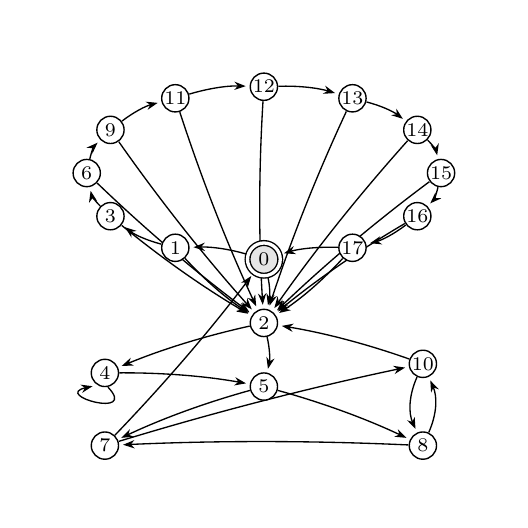
\begin{tikzpicture}[x=1cm,y=1cm,
  f1atlas state/.style={circle,draw=black,fill=white,line width=.5pt,inner sep=0pt,font=\fontsize{7}{8}\selectfont},
  f1atlas root/.style={f1atlas state,double,double distance=.42mm},
  f1atlas port0/.style={-{Stealth[length=1.45mm,width=1.05mm]},draw=black,line width=.48pt},
  f1atlas port1/.style={f1atlas port0},
  f1atlas label/.style={font=\fontsize{6}{7}\selectfont,fill=white,inner sep=.4pt}
]
\path[use as bounding box] (-3,-3) rectangle (3,3);
% edge 0 0 1
\draw[f1atlas port0] (-0.21001,0.12062) .. controls (-0.43704,0.18864) and (-0.66515,0.21904) .. (-0.89435,0.21182);
% edge 0 1 2
\draw[f1atlas port1] (0.04885,-0.15603) .. controls (0.07782,-0.28278) and (0.07868,-0.40578) .. (0.05142,-0.52503);
% edge 1 0 2
\draw[f1atlas port0] (-1.00015,0.06855) .. controls (-0.74820,-0.20589) and (-0.47919,-0.43664) .. (-0.19314,-0.62370);
% edge 1 1 3
\draw[f1atlas port1] (-1.30367,0.25102) .. controls (-1.48603,0.29846) and (-1.63986,0.37002) .. (-1.76515,0.46571);
% edge 2 0 4
\draw[f1atlas port0] (-0.18027,-0.78984) .. controls (-0.75162,-0.91611) and (-1.29350,-1.08502) .. (-1.80592,-1.29656);
% edge 2 1 5
\draw[f1atlas port1] (0.04114,-0.92997) .. controls (0.07525,-1.07922) and (0.07868,-1.21347) .. (0.05142,-1.33272);
% edge 3 0 2
\draw[f1atlas port0] (-1.80565,0.48890) .. controls (-1.28655,0.06437) and (-0.75103,-0.30969) .. (-0.19908,-0.63328);
% edge 3 1 6
\draw[f1atlas port1] (-2.07968,0.73573) .. controls (-2.14667,0.80213) and (-2.18697,0.86636) .. (-2.20058,0.92843);
% edge 4 0 4
\draw[f1atlas port0] (-1.98070,-1.56516) .. controls (-1.59080,-1.97187) and (-2.68847,-1.66841) .. (-2.17649,-1.55351);
% edge 4 1 5
\draw[f1atlas port1] (-1.83462,-1.38363) .. controls (-1.27936,-1.38067) and (-0.74355,-1.42519) .. (-0.22719,-1.51721);
% edge 5 0 7
\draw[f1atlas port0] (-0.17792,-1.60696) .. controls (-0.75381,-1.76643) and (-1.29802,-1.96716) .. (-1.81055,-2.20916);
% edge 5 1 8
\draw[f1atlas port1] (0.17792,-1.60696) .. controls (0.75381,-1.76643) and (1.29802,-1.96716) .. (1.81055,-2.20916);
% edge 6 0 2
\draw[f1atlas port0] (-2.11680,1.02602) .. controls (-1.49535,0.42964) and (-0.85146,-0.11644) .. (-0.18514,-0.61224);
% edge 6 1 9
\draw[f1atlas port1] (-2.21046,1.33418) .. controls (-2.19026,1.42631) and (-2.15759,1.49474) .. (-2.11246,1.53947);
% edge 7 0 0
\draw[f1atlas port0] (-1.89126,-2.17463) .. controls (-1.25669,-1.51483) and (-0.67962,-0.84129) .. (-0.16004,-0.15401);
% edge 7 1 10
\draw[f1atlas port1] (-1.84264,-2.25385) .. controls (-0.62954,-1.88399) and (0.58248,-1.57163) .. (1.79341,-1.31676);
% edge 8 0 7
\draw[f1atlas port0] (1.83481,-2.29926) .. controls (0.61160,-2.24334) and (-0.59623,-2.24264) .. (-1.78870,-2.29715);
% edge 8 1 10
\draw[f1atlas port1] (2.09421,-2.13899) .. controls (2.19807,-1.90530) and (2.20432,-1.68568) .. (2.11296,-1.48011);
% edge 9 0 2
\draw[f1atlas port0] (-1.84240,1.55088) .. controls (-1.31183,0.79598) and (-0.74902,0.08632) .. (-0.15396,-0.57810);
% edge 9 1 11
\draw[f1atlas port1] (-1.80183,1.81397) .. controls (-1.65208,1.92834) and (-1.50092,2.00536) .. (-1.34834,2.04505);
% edge 10 0 2
\draw[f1atlas port0] (1.84518,-1.20766) .. controls (1.30346,-1.01603) and (0.76430,-0.87599) .. (0.22770,-0.78753);
% edge 10 1 8
\draw[f1atlas port1] (1.94425,-1.43793) .. controls (1.84039,-1.67162) and (1.83414,-1.89125) .. (1.92551,-2.09681);
% edge 11 0 2
\draw[f1atlas port0] (-1.06772,1.92764) .. controls (-0.78816,1.07102) and (-0.46471,0.24821) .. (-0.09740,-0.54079);
% edge 11 1 12
\draw[f1atlas port1] (-0.94815,2.15613) .. controls (-0.69902,2.23078) and (-0.45985,2.26449) .. (-0.23065,2.25727);
% edge 12 0 2
\draw[f1atlas port0] (-0.01134,2.06573) .. controls (-0.06532,1.18858) and (-0.06626,0.32678) .. (-0.01417,-0.51967);
% edge 12 1 13
\draw[f1atlas port1] (0.18452,2.25581) .. controls (0.44447,2.26401) and (0.68428,2.23519) .. (0.90394,2.16938);
% edge 13 0 2
\draw[f1atlas port0] (1.04708,1.93578) .. controls (0.66678,1.11888) and (0.34162,0.29675) .. (0.07160,-0.53062);
% edge 13 1 14
\draw[f1atlas port1] (1.30367,2.05667) .. controls (1.48603,2.00923) and (1.63986,1.93767) .. (1.76515,1.84199);
% edge 14 0 2
\draw[f1atlas port0] (1.82539,1.56440) .. controls (1.20980,0.87706) and (0.64557,0.16853) .. (0.13270,-0.56120);
% edge 14 1 15
\draw[f1atlas port1] (2.07968,1.57196) .. controls (2.14667,1.50557) and (2.18697,1.44133) .. (2.20058,1.37926);
% edge 15 0 2
\draw[f1atlas port0] (2.10189,1.04364) .. controls (1.41088,0.52947) and (0.76575,-0.01515) .. (0.16650,-0.59022);
% edge 15 1 16
\draw[f1atlas port1] (2.21046,0.97351) .. controls (2.19026,0.88139) and (2.15759,0.81296) .. (2.11246,0.76822);
% edge 16 0 2
\draw[f1atlas port0] (1.78930,0.51240) .. controls (1.21080,0.17324) and (0.67392,-0.19887) .. (0.17864,-0.60391);
% edge 16 1 17
\draw[f1atlas port1] (1.80183,0.49372) .. controls (1.65208,0.37936) and (1.50092,0.30233) .. (1.34834,0.26264);
% edge 17 0 0
\draw[f1atlas port0] (0.94048,0.21036) .. controls (0.68053,0.21856) and (0.45177,0.19306) .. (0.25422,0.13386);
% edge 17 1 2
\draw[f1atlas port1] (1.00015,0.06855) .. controls (0.74820,-0.20589) and (0.47919,-0.43664) .. (0.19314,-0.62370);
% state 0
\node[f1atlas root,minimum size=4.1538mm,fill=black!10] (q0) at (0.00000,0.05769) {$ 0 $};
% state 1
\node[f1atlas state,minimum size=3.4615mm] (q1) at (-1.12500,0.20455) {$ 1 $};
% state 2
\node[f1atlas state,minimum size=3.4615mm] (q2) at (0.00000,-0.75000) {$ 2 $};
% state 3
\node[f1atlas state,minimum size=3.4615mm] (q3) at (-1.94856,0.60577) {$ 3 $};
% state 4
\node[f1atlas state,minimum size=3.4615mm] (q4) at (-2.01923,-1.38462) {$ 4 $};
% state 5
\node[f1atlas state,minimum size=3.4615mm] (q5) at (0.00000,-1.55769) {$ 5 $};
% state 6
\node[f1atlas state,minimum size=3.4615mm] (q6) at (-2.25000,1.15385) {$ 6 $};
% state 7
\node[f1atlas state,minimum size=3.4615mm] (q7) at (-2.01923,-2.30769) {$ 7 $};
% state 8
\node[f1atlas state,minimum size=3.4615mm] (q8) at (2.01923,-2.30769) {$ 8 $};
% state 9
\node[f1atlas state,minimum size=3.4615mm] (q9) at (-1.94856,1.70192) {$ 9 $};
% state 10
\node[f1atlas state,minimum size=3.4615mm] (q10) at (2.01923,-1.26923) {$ 10 $};
% state 11
\node[f1atlas state,minimum size=3.4615mm] (q11) at (-1.12500,2.10314) {$ 11 $};
% state 12
\node[f1atlas state,minimum size=3.4615mm] (q12) at (-0.00000,2.25000) {$ 12 $};
% state 13
\node[f1atlas state,minimum size=3.4615mm] (q13) at (1.12500,2.10314) {$ 13 $};
% state 14
\node[f1atlas state,minimum size=3.4615mm] (q14) at (1.94856,1.70192) {$ 14 $};
% state 15
\node[f1atlas state,minimum size=3.4615mm] (q15) at (2.25000,1.15385) {$ 15 $};
% state 16
\node[f1atlas state,minimum size=3.4615mm] (q16) at (1.94856,0.60577) {$ 16 $};
% state 17
\node[f1atlas state,minimum size=3.4615mm] (q17) at (1.12500,0.20455) {$ 17 $};
\end{tikzpicture}
}\par
\small\textbf{(a)} Example start: $0$. Proved $H\ge34$.\\Exact score and global maximum unresolved.\par\end{minipage}
\clearpage
{\LARGE\bfseries $m=19$}\par\vspace{3mm}
\textbf{Constructive lower-bound example.} The indicated start gives $H\ge34$ by a static-mask projection onto a certified seven-state maximizer. This graph has not been certified globally optimal; its exact score is unresolved.\par\vspace{3mm}
\begin{minipage}[t]{.94\textwidth}\centering
\resizebox{10.3cm}{!}{% Family 1 rooted seed, m=19; key=0102020304050206040507080209001007100211020802120213021402150216021702180002.
% Requires \usepackage{tikz} and \usetikzlibrary{arrows.meta}.
% Score and global-maximality metadata belong in the surrounding caption.
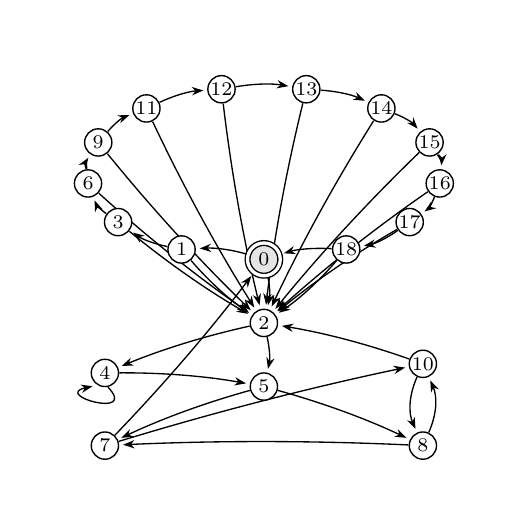
\begin{tikzpicture}[x=1cm,y=1cm,
  f1atlas state/.style={circle,draw=black,fill=white,line width=.5pt,inner sep=0pt,font=\fontsize{7}{8}\selectfont},
  f1atlas root/.style={f1atlas state,double,double distance=.42mm},
  f1atlas port0/.style={-{Stealth[length=1.45mm,width=1.05mm]},draw=black,line width=.48pt},
  f1atlas port1/.style={f1atlas port0},
  f1atlas label/.style={font=\fontsize{6}{7}\selectfont,fill=white,inner sep=.4pt}
]
\path[use as bounding box] (-3,-3) rectangle (3,3);
% edge 0 0 1
\draw[f1atlas port0] (-0.20988,0.12102) .. controls (-0.41117,0.18175) and (-0.61294,0.20665) .. (-0.81519,0.19571);
% edge 0 1 2
\draw[f1atlas port1] (0.04885,-0.15603) .. controls (0.07782,-0.28278) and (0.07868,-0.40578) .. (0.05142,-0.52503);
% edge 1 0 2
\draw[f1atlas port0] (-0.92513,0.04338) .. controls (-0.69790,-0.22037) and (-0.45311,-0.44154) .. (-0.19076,-0.62014);
% edge 1 1 3
\draw[f1atlas port1] (-1.22656,0.21996) .. controls (-1.39902,0.25496) and (-1.54456,0.31433) .. (-1.66319,0.39807);
% edge 2 0 4
\draw[f1atlas port0] (-0.18027,-0.78984) .. controls (-0.75162,-0.91611) and (-1.29350,-1.08502) .. (-1.80592,-1.29656);
% edge 2 1 5
\draw[f1atlas port1] (0.04114,-0.92997) .. controls (0.07525,-1.07922) and (0.07868,-1.21347) .. (0.05142,-1.33272);
% edge 3 0 2
\draw[f1atlas port0] (-1.70898,0.41406) .. controls (-1.22191,0.01447) and (-0.71887,-0.33510) .. (-0.19987,-0.63465);
% edge 3 1 6
\draw[f1atlas port1] (-2.00190,0.63853) .. controls (-2.07763,0.69267) and (-2.12684,0.74876) .. (-2.14954,0.80680);
% edge 4 0 4
\draw[f1atlas port0] (-1.98070,-1.56516) .. controls (-1.59080,-1.97187) and (-2.68847,-1.66841) .. (-2.17649,-1.55351);
% edge 4 1 5
\draw[f1atlas port1] (-1.83462,-1.38363) .. controls (-1.27936,-1.38067) and (-0.74355,-1.42519) .. (-0.22719,-1.51721);
% edge 5 0 7
\draw[f1atlas port0] (-0.17792,-1.60696) .. controls (-0.75381,-1.76643) and (-1.29802,-1.96716) .. (-1.81055,-2.20916);
% edge 5 1 8
\draw[f1atlas port1] (0.17792,-1.60696) .. controls (0.75381,-1.76643) and (1.29802,-1.96716) .. (1.81055,-2.20916);
% edge 6 0 2
\draw[f1atlas port0] (-2.09667,0.89788) .. controls (-1.48167,0.34166) and (-0.84600,-0.16383) .. (-0.18969,-0.61857);
% edge 6 1 9
\draw[f1atlas port1] (-2.24964,1.20564) .. controls (-2.25539,1.27152) and (-2.24864,1.31929) .. (-2.22939,1.34895);
% edge 7 0 0
\draw[f1atlas port0] (-1.89126,-2.17463) .. controls (-1.25669,-1.51483) and (-0.67962,-0.84129) .. (-0.16004,-0.15401);
% edge 7 1 10
\draw[f1atlas port1] (-1.84264,-2.25385) .. controls (-0.62954,-1.88399) and (0.58248,-1.57163) .. (1.79341,-1.31676);
% edge 8 0 7
\draw[f1atlas port0] (1.83481,-2.29926) .. controls (0.61160,-2.24334) and (-0.59623,-2.24264) .. (-1.78870,-2.29715);
% edge 8 1 10
\draw[f1atlas port1] (2.09421,-2.13899) .. controls (2.19807,-1.90530) and (2.20432,-1.68568) .. (2.11296,-1.48011);
% edge 9 0 2
\draw[f1atlas port0] (-1.98724,1.39937) .. controls (-1.40902,0.68903) and (-0.80188,0.02607) .. (-0.16583,-0.58951);
% edge 9 1 11
\draw[f1atlas port1] (-1.98283,1.68202) .. controls (-1.89503,1.78324) and (-1.80307,1.85266) .. (-1.70694,1.89026);
% edge 10 0 2
\draw[f1atlas port0] (1.84518,-1.20766) .. controls (1.30346,-1.01603) and (0.76430,-0.87599) .. (0.22770,-0.78753);
% edge 10 1 8
\draw[f1atlas port1] (1.94425,-1.43793) .. controls (1.84039,-1.67162) and (1.83414,-1.89125) .. (1.92551,-2.09681);
% edge 11 0 2
\draw[f1atlas port0] (-1.41311,1.80743) .. controls (-1.02235,0.98103) and (-0.59220,0.19371) .. (-0.12266,-0.55453);
% edge 11 1 12
\draw[f1atlas port1] (-1.32466,2.05225) .. controls (-1.13363,2.14120) and (-0.94832,2.19151) .. (-0.76874,2.20318);
% edge 12 0 2
\draw[f1atlas port0] (-0.51666,2.03482) .. controls (-0.41226,1.15667) and (-0.25837,0.30311) .. (-0.05499,-0.52588);
% edge 12 1 13
\draw[f1atlas port1] (-0.35650,2.24934) .. controls (-0.11883,2.29008) and (0.10367,2.29268) .. (0.31101,2.25714);
% edge 13 0 2
\draw[f1atlas port0] (0.49447,2.03885) .. controls (0.28376,1.17998) and (0.12802,0.32675) .. (0.02724,-0.52084);
% edge 13 1 14
\draw[f1atlas port1] (0.72269,2.20617) .. controls (0.93297,2.19250) and (1.11968,2.14769) .. (1.28282,2.07173);
% edge 14 0 2
\draw[f1atlas port0] (1.39390,1.81795) .. controls (0.90800,1.04365) and (0.47625,0.25721) .. (0.09865,-0.54138);
% edge 14 1 15
\draw[f1atlas port1] (1.66396,1.90707) .. controls (1.78874,1.85826) and (1.88495,1.79486) .. (1.95258,1.71688);
% edge 15 0 2
\draw[f1atlas port0] (1.97113,1.41416) .. controls (1.31296,0.77718) and (0.70448,0.11545) .. (0.14568,-0.57103);
% edge 15 1 16
\draw[f1atlas port1] (2.20427,1.38767) .. controls (2.24026,1.33220) and (2.25672,1.28684) .. (2.25365,1.25162);
% edge 16 0 2
\draw[f1atlas port0] (2.08185,0.91658) .. controls (1.40024,0.44431) and (0.76334,-0.05962) .. (0.17115,-0.59521);
% edge 16 1 17
\draw[f1atlas port1] (2.16635,0.84979) .. controls (2.13245,0.76309) and (2.09014,0.70161) .. (2.03944,0.66537);
% edge 17 0 2
\draw[f1atlas port0] (1.69182,0.43888) .. controls (1.14616,0.12395) and (0.64169,-0.22355) .. (0.17841,-0.60363);
% edge 17 1 18
\draw[f1atlas port1] (1.70089,0.42469) .. controls (1.55713,0.32320) and (1.41410,0.25802) .. (1.27179,0.22914);
% edge 18 0 0
\draw[f1atlas port0] (0.86128,0.19322) .. controls (0.62830,0.20582) and (0.42590,0.18620) .. (0.25407,0.13435);
% edge 18 1 2
\draw[f1atlas port1] (0.92513,0.04338) .. controls (0.69790,-0.22037) and (0.45311,-0.44154) .. (0.19076,-0.62014);
% state 0
\node[f1atlas root,minimum size=4.1538mm,fill=black!10] (q0) at (0.00000,0.05769) {$ 0 $};
% state 1
\node[f1atlas state,minimum size=3.4615mm] (q1) at (-1.04563,0.18325) {$ 1 $};
% state 2
\node[f1atlas state,minimum size=3.4615mm] (q2) at (0.00000,-0.75000) {$ 2 $};
% state 3
\node[f1atlas state,minimum size=3.4615mm] (q3) at (-1.85171,0.53116) {$ 3 $};
% state 4
\node[f1atlas state,minimum size=3.4615mm] (q4) at (-2.01923,-1.38462) {$ 4 $};
% state 5
\node[f1atlas state,minimum size=3.4615mm] (q5) at (0.00000,-1.55769) {$ 5 $};
% state 6
\node[f1atlas state,minimum size=3.4615mm] (q6) at (-2.23359,1.02172) {$ 6 $};
% state 7
\node[f1atlas state,minimum size=3.4615mm] (q7) at (-2.01923,-2.30769) {$ 7 $};
% state 8
\node[f1atlas state,minimum size=3.4615mm] (q8) at (2.01923,-2.30769) {$ 8 $};
% state 9
\node[f1atlas state,minimum size=3.4615mm] (q9) at (-2.10379,1.54255) {$ 9 $};
% state 10
\node[f1atlas state,minimum size=3.4615mm] (q10) at (2.01923,-1.26923) {$ 10 $};
% state 11
\node[f1atlas state,minimum size=3.4615mm] (q11) at (-1.49203,1.97433) {$ 11 $};
% state 12
\node[f1atlas state,minimum size=3.4615mm] (q12) at (-0.53846,2.21815) {$ 12 $};
% state 13
\node[f1atlas state,minimum size=3.4615mm] (q13) at (0.53846,2.21815) {$ 13 $};
% state 14
\node[f1atlas state,minimum size=3.4615mm] (q14) at (1.49203,1.97433) {$ 14 $};
% state 15
\node[f1atlas state,minimum size=3.4615mm] (q15) at (2.10379,1.54255) {$ 15 $};
% state 16
\node[f1atlas state,minimum size=3.4615mm] (q16) at (2.23359,1.02172) {$ 16 $};
% state 17
\node[f1atlas state,minimum size=3.4615mm] (q17) at (1.85171,0.53116) {$ 17 $};
% state 18
\node[f1atlas state,minimum size=3.4615mm] (q18) at (1.04563,0.18325) {$ 18 $};
\end{tikzpicture}
}\par
\small\textbf{(a)} Example start: $0$. Proved $H\ge34$.\\Exact score and global maximum unresolved.\par\end{minipage}
\clearpage
{\LARGE\bfseries $m=20$}\par\vspace{3mm}
\textbf{Constructive lower-bound example.} The indicated start gives $H\ge34$ by a static-mask projection onto a certified seven-state maximizer. This graph has not been certified globally optimal; its exact score is unresolved.\par\vspace{3mm}
\begin{minipage}[t]{.94\textwidth}\centering
\resizebox{10.3cm}{!}{% Family 1 rooted seed, m=20; key=01020203040502060405070802090010071002110208021202130214021502160217021802190002.
% Requires \usepackage{tikz} and \usetikzlibrary{arrows.meta}.
% Score and global-maximality metadata belong in the surrounding caption.
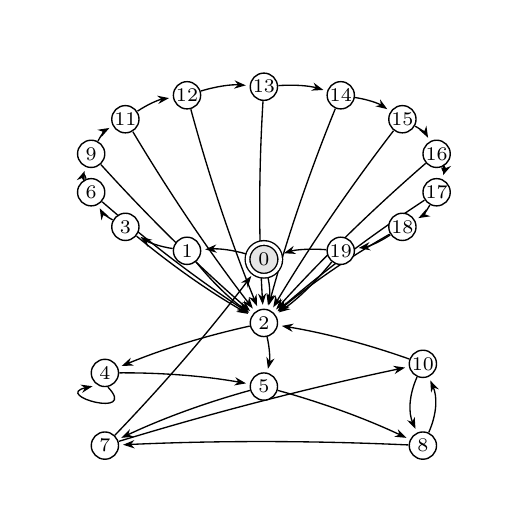
\begin{tikzpicture}[x=1cm,y=1cm,
  f1atlas state/.style={circle,draw=black,fill=white,line width=.5pt,inner sep=0pt,font=\fontsize{7}{8}\selectfont},
  f1atlas root/.style={f1atlas state,double,double distance=.42mm},
  f1atlas port0/.style={-{Stealth[length=1.45mm,width=1.05mm]},draw=black,line width=.48pt},
  f1atlas port1/.style={f1atlas port0},
  f1atlas label/.style={font=\fontsize{6}{7}\selectfont,fill=white,inner sep=.4pt}
]
\path[use as bounding box] (-3,-3) rectangle (3,3);
% edge 0 0 1
\draw[f1atlas port0] (-0.20966,0.12175) .. controls (-0.38850,0.17639) and (-0.56732,0.19699) .. (-0.74612,0.18355);
% edge 0 1 2
\draw[f1atlas port1] (0.04885,-0.15603) .. controls (0.07782,-0.28278) and (0.07868,-0.40578) .. (0.05142,-0.52503);
% edge 1 0 2
\draw[f1atlas port0] (-0.86014,0.02270) .. controls (-0.65424,-0.23189) and (-0.43028,-0.44497) .. (-0.18826,-0.61654);
% edge 1 1 3
\draw[f1atlas port1] (-1.15866,0.19460) .. controls (-1.32029,0.21972) and (-1.45640,0.26906) .. (-1.56697,0.34260);
% edge 2 0 4
\draw[f1atlas port0] (-0.18027,-0.78984) .. controls (-0.75162,-0.91611) and (-1.29350,-1.08502) .. (-1.80592,-1.29656);
% edge 2 1 5
\draw[f1atlas port1] (0.04114,-0.92997) .. controls (0.07525,-1.07922) and (0.07868,-1.21347) .. (0.05142,-1.33272);
% edge 3 0 2
\draw[f1atlas port0] (-1.61704,0.35253) .. controls (-1.16046,-0.02625) and (-0.68819,-0.35550) .. (-0.20021,-0.63523);
% edge 3 1 6
\draw[f1atlas port1] (-1.92106,0.55906) .. controls (-2.00169,0.60320) and (-2.05637,0.65226) .. (-2.08512,0.70624);
% edge 4 0 4
\draw[f1atlas port0] (-1.98070,-1.56516) .. controls (-1.59080,-1.97187) and (-2.68847,-1.66841) .. (-2.17649,-1.55351);
% edge 4 1 5
\draw[f1atlas port1] (-1.83462,-1.38363) .. controls (-1.27936,-1.38067) and (-0.74355,-1.42519) .. (-0.22719,-1.51721);
% edge 5 0 7
\draw[f1atlas port0] (-0.17792,-1.60696) .. controls (-0.75381,-1.76643) and (-1.29802,-1.96716) .. (-1.81055,-2.20916);
% edge 5 1 8
\draw[f1atlas port1] (0.17792,-1.60696) .. controls (0.75381,-1.76643) and (1.29802,-1.96716) .. (1.81055,-2.20916);
% edge 6 0 2
\draw[f1atlas port0] (-2.05416,0.78892) .. controls (-1.45305,0.26721) and (-0.83264,-0.20356) .. (-0.19293,-0.62338);
% edge 6 1 9
\draw[f1atlas port1] (-2.25893,1.08259) .. controls (-2.27691,1.13010) and (-2.28235,1.16321) .. (-2.27527,1.18193);
% edge 7 0 0
\draw[f1atlas port0] (-1.89126,-2.17463) .. controls (-1.25669,-1.51483) and (-0.67962,-0.84129) .. (-0.16004,-0.15401);
% edge 7 1 10
\draw[f1atlas port1] (-1.84264,-2.25385) .. controls (-0.62954,-1.88399) and (0.58248,-1.57163) .. (1.79341,-1.31676);
% edge 8 0 7
\draw[f1atlas port0] (1.83481,-2.29926) .. controls (0.61160,-2.24334) and (-0.59623,-2.24264) .. (-1.78870,-2.29715);
% edge 8 1 10
\draw[f1atlas port1] (2.09421,-2.13899) .. controls (2.19807,-1.90530) and (2.20432,-1.68568) .. (2.11296,-1.48011);
% edge 9 0 2
\draw[f1atlas port0] (-2.06967,1.26092) .. controls (-1.46414,0.59226) and (-0.83234,-0.02763) .. (-0.17429,-0.59874);
% edge 9 1 11
\draw[f1atlas port1] (-2.10681,1.56071) .. controls (-2.06361,1.64185) and (-2.01518,1.69710) .. (-1.96154,1.72647);
% edge 10 0 2
\draw[f1atlas port0] (1.84518,-1.20766) .. controls (1.30346,-1.01603) and (0.76430,-0.87599) .. (0.22770,-0.78753);
% edge 10 1 8
\draw[f1atlas port1] (1.94425,-1.43793) .. controls (1.84039,-1.67162) and (1.83414,-1.89125) .. (1.92551,-2.09681);
% edge 11 0 2
\draw[f1atlas port0] (-1.66449,1.67877) .. controls (-1.19209,0.88742) and (-0.68419,0.13878) .. (-0.14077,-0.56714);
% edge 11 1 12
\draw[f1atlas port1] (-1.60540,1.93953) .. controls (-1.46921,2.03012) and (-1.33550,2.08561) .. (-1.20427,2.10600);
% edge 12 0 2
\draw[f1atlas port0] (-0.92785,1.96329) .. controls (-0.69300,1.09856) and (-0.41268,0.26539) .. (-0.08689,-0.53621);
% edge 12 1 13
\draw[f1atlas port1] (-0.79968,2.19539) .. controls (-0.59877,2.25677) and (-0.40892,2.28074) .. (-0.23012,2.26730);
% edge 13 0 2
\draw[f1atlas port0] (-0.01134,2.06573) .. controls (-0.06532,1.18858) and (-0.06626,0.32678) .. (-0.01417,-0.51967);
% edge 13 1 14
\draw[f1atlas port1] (0.18410,2.26384) .. controls (0.39358,2.27959) and (0.58406,2.26127) .. (0.75554,2.20888);
% edge 14 0 2
\draw[f1atlas port0] (0.90673,1.97042) .. controls (0.56935,1.14031) and (0.28727,0.30774) .. (0.06048,-0.52730);
% edge 14 1 15
\draw[f1atlas port1] (1.15866,2.11309) .. controls (1.32029,2.08797) and (1.45640,2.03864) .. (1.56697,1.96509);
% edge 15 0 2
\draw[f1atlas port0] (1.64651,1.69100) .. controls (1.08432,0.96070) and (0.57491,0.21308) .. (0.11829,-0.55185);
% edge 15 1 16
\draw[f1atlas port1] (1.92106,1.74863) .. controls (2.00169,1.70449) and (2.05637,1.65543) .. (2.08512,1.60145);
% edge 16 0 2
\draw[f1atlas port0] (2.05416,1.27676) .. controls (1.37286,0.68548) and (0.73978,0.06691) .. (0.15490,-0.57895);
% edge 16 1 17
\draw[f1atlas port1] (2.25893,1.22510) .. controls (2.27691,1.17760) and (2.28235,1.14448) .. (2.27527,1.12576);
% edge 17 0 2
\draw[f1atlas port0] (2.03924,0.80864) .. controls (1.37381,0.37193) and (0.75216,-0.09720) .. (0.17428,-0.59874);
% edge 17 1 18
\draw[f1atlas port1] (2.10681,0.74698) .. controls (2.06361,0.66584) and (2.01518,0.61059) .. (1.96154,0.58122);
% edge 18 0 2
\draw[f1atlas port0] (1.59895,0.37859) .. controls (1.08428,0.08356) and (0.61050,-0.24352) .. (0.17761,-0.60266);
% edge 18 1 19
\draw[f1atlas port1] (1.60540,0.36816) .. controls (1.46921,0.27758) and (1.33550,0.22209) .. (1.20427,0.20169);
% edge 19 0 0
\draw[f1atlas port0] (0.79214,0.18009) .. controls (0.58266,0.19584) and (0.40321,0.18089) .. (0.25380,0.13524);
% edge 19 1 2
\draw[f1atlas port1] (0.86014,0.02270) .. controls (0.65424,-0.23189) and (0.43028,-0.44497) .. (0.18826,-0.61654);
% state 0
\node[f1atlas root,minimum size=4.1538mm,fill=black!10] (q0) at (0.00000,0.05769) {$ 0 $};
% state 1
\node[f1atlas state,minimum size=3.4615mm] (q1) at (-0.97624,0.16625) {$ 1 $};
% state 2
\node[f1atlas state,minimum size=3.4615mm] (q2) at (0.00000,-0.75000) {$ 2 $};
% state 3
\node[f1atlas state,minimum size=3.4615mm] (q3) at (-1.75912,0.47041) {$ 3 $};
% state 4
\node[f1atlas state,minimum size=3.4615mm] (q4) at (-2.01923,-1.38462) {$ 4 $};
% state 5
\node[f1atlas state,minimum size=3.4615mm] (q5) at (0.00000,-1.55769) {$ 5 $};
% state 6
\node[f1atlas state,minimum size=3.4615mm] (q6) at (-2.19359,0.90993) {$ 6 $};
% state 7
\node[f1atlas state,minimum size=3.4615mm] (q7) at (-2.01923,-2.30769) {$ 7 $};
% state 8
\node[f1atlas state,minimum size=3.4615mm] (q8) at (2.01923,-2.30769) {$ 8 $};
% state 9
\node[f1atlas state,minimum size=3.4615mm] (q9) at (-2.19359,1.39776) {$ 9 $};
% state 10
\node[f1atlas state,minimum size=3.4615mm] (q10) at (2.01923,-1.26923) {$ 10 $};
% state 11
\node[f1atlas state,minimum size=3.4615mm] (q11) at (-1.75912,1.83729) {$ 11 $};
% state 12
\node[f1atlas state,minimum size=3.4615mm] (q12) at (-0.97624,2.14145) {$ 12 $};
% state 13
\node[f1atlas state,minimum size=3.4615mm] (q13) at (-0.00000,2.25000) {$ 13 $};
% state 14
\node[f1atlas state,minimum size=3.4615mm] (q14) at (0.97624,2.14145) {$ 14 $};
% state 15
\node[f1atlas state,minimum size=3.4615mm] (q15) at (1.75912,1.83729) {$ 15 $};
% state 16
\node[f1atlas state,minimum size=3.4615mm] (q16) at (2.19359,1.39776) {$ 16 $};
% state 17
\node[f1atlas state,minimum size=3.4615mm] (q17) at (2.19359,0.90993) {$ 17 $};
% state 18
\node[f1atlas state,minimum size=3.4615mm] (q18) at (1.75912,0.47041) {$ 18 $};
% state 19
\node[f1atlas state,minimum size=3.4615mm] (q19) at (0.97624,0.16625) {$ 19 $};
\end{tikzpicture}
}\par
\small\textbf{(a)} Example start: $0$. Proved $H\ge34$.\\Exact score and global maximum unresolved.\par\end{minipage}
\end{document}
